% Chapter 7 of Volume III: the cancellation ledger, the Fejer criterion and the oscillator. Sources: chG_bondesson.tex 444-1050 (kept whole), ch9_path_to_rh.tex 150-182; reports U09 (M1 to M13), Astra V3A (rows 444-1050); verification W4 (V13); new mathematics from misc/vol3/ledger (SYNTHESIS, opus_AB, opus_CD, opus_smooth, Astra V3L sections 1 to 9, num/results). 17 Nov 2026.
\label{bo:ch:ledger}
\providecommand{\dd}{\mathrm{d}}

This chapter keeps the whole of Bondesson's ledger and oscillator material from an unrefereed note of Polson (November 2026), with the corrections of the referees and the verification runs, and adds the mathematics that two further readings of the ledger produced. The results of Volumes I and II that it touches are cited where they occur, in particular Proposition~\ref{yo:prop:tent} and Theorem~\ref{yo:thm:D} (the oscillator at $\alpha=\frac12$ in the form $D=2f$), Lemma~\ref{pol:lem:Bbound} and Theorem~\ref{pol:thm:almostall} (positivity at the origin and at almost all heights).

\paragraph{Conventions.} The Riemann function is $\xi(s)=\frac12s(s-1)\pi^{-s/2}\Gamma(s/2)\zeta(s)=(s-1)\pi^{-s/2}\Gamma(1+\frac s2)\zeta(s)$, the nontrivial zeros $\rho=\beta+i\gamma$ are counted with multiplicity, and $\Theta=\sup\beta$. We write $s=\alpha+it$ and $\delta=\alpha-\frac12$. The Thorin density at level $\alpha$, in the ordinate variable $t$, is $u_\alpha(t)=\pi^{-1}\Re\,\xi'/\xi(\alpha+it)$ (Theorem~\ref{thm:poisson}). Chebyshev's function is $\Psi(y)=\sum_{n\le y}\Lambda(n)$, so that $R(y)=\Psi(y)-y$ is the error in the prime number theorem, $R(1)=-1$ and $E(y)=R(y)/\sqrt y$. The digamma function is $\psi$. Put
\[
G(s)=-\tfrac12\log\pi+\tfrac12\psi\bigl(1+\tfrac s2\bigr),\qquad F(s)=-\frac{\zeta'}{\zeta}(s)-\frac1{s-1}.
\]
$F$ is meromorphic on $\mathbb C$, regular at $s=1$ with $F(1)=-\gamma_E$, and has simple poles exactly at the zeros of $\zeta$. Logarithmic differentiation gives
\begin{equation}\label{bo:eq:xi}
\frac{\xi'}{\xi}(s)=G(s)-F(s)=\sum_\rho\frac1{s-\rho},
\end{equation}
the sum in symmetric order, its real part absolutely convergent after pairing $\rho$ with $1-\bar\rho$. In the oscillator sections the atoms of the spectral measure sit at $\gamma^{-2}$, the chart of this volume. Two constants recur:
\[
q=\frac{\xi''}{\xi}\Bigl(\frac12\Bigr)=0.0462099862308,\qquad M=2q=4\sum_{\gamma>0}\gamma^{-2}=0.0924199724617,
\]
where $M=4\sum_{\gamma>0}\gamma^{-2}$ is the value of $2q$ under RH, and $\frac14\psi'(\frac54)=\sum_{k\ge1}(2k+\frac12)^{-2}=0.2993322886$.

\section{The ledger}\label{bo:sec:ledger}

Bondesson's method writes each factor of $\xi$ as a sum of nonnegative $2\sin^2$ blocks and a drift. Above level $1$ every block is finite and only the pole pays at $t=0$. This section asks what the same bookkeeping says in the strip: which blocks must cancel for $u_\alpha$ to be positive, how finely, and at what cost.

The archimedean block is
\begin{multline}\label{bo:eq:B}
B_\alpha(t)=\Re G(s)-G(\alpha)=\frac12\Re\Bigl[\psi\bigl(1+\tfrac s2\bigr)-\psi\bigl(1+\tfrac\alpha2\bigr)\Bigr]\\=\sum_{k\ge1}\frac{t^2}{(\alpha+2k)\bigl((\alpha+2k)^2+t^2\bigr)}.
\end{multline}
It is the $2\sin^2$ transform $\int_0^\infty(1-\cos tw)\,b_\alpha(w)\,\dd w$ of the positive density $b_\alpha(w)=e^{-(\alpha+2)w}/(1-e^{-2w})$ (sum $\frac1c-\Re\frac1{c+it}=\int_0^\infty(1-\cos tw)e^{-cw}\dd w$ over $c=\alpha+2k$). So $B_\alpha\ge0$, $B_\alpha(0)=0$, and $B_\alpha(t)=\frac12\log\frac t2-\frac12\psi(1+\frac\alpha2)+O(t^{-2})$. The factor $s$ of $\xi$ is inside this block, because it turns $\Gamma(s/2)$ into $\Gamma(1+s/2)$.

\begin{theorem}[Cancellation ledger]\label{bo:thm:ledger}
Let $\alpha>\Theta$. For every real $t$ the improper Stieltjes integral
\[
J_\alpha(t)=\int_1^\infty\bigl(1-\cos(t\log y)\bigr)\,y^{-\alpha}\dd R(y)=\lim_{Y\to\infty}\int_{[1,Y]}\bigl(1-\cos(t\log y)\bigr)\,y^{-\alpha}\dd R(y)
\]
exists, equals $F(\alpha)-\Re F(\alpha+it)$, and
\begin{equation}\label{bo:eq:ledger}
\pi\,u_\alpha(t)=B_\alpha(t)+\frac{\xi'}{\xi}(\alpha)+J_\alpha(t),\qquad B_\alpha(0)=J_\alpha(0)=0 .
\end{equation}
In addition:
\begin{enumerate}
\item for $\alpha>1$ both blocks converge absolutely, $J_\alpha=P_\alpha-Q_\alpha$ with $P_\alpha(t)=\sum_n\Lambda(n)n^{-\alpha}(1-\cos(t\log n))\in[0,-2\frac{\zeta'}{\zeta}(\alpha)]$ and $Q_\alpha(t)=\frac{t^2}{(\alpha-1)((\alpha-1)^2+t^2)}$;
\item at $\alpha=1$ the identity holds unconditionally although both blocks diverge;
\item for $\Theta<\alpha<1$ and $t\ne0$ both blocks diverge, each of exact order $Y^{1-\alpha}$, and only their difference converges;
\item for $\alpha>\Theta$ one has $u_\alpha(t)>0$ for every $t$, and for $\alpha<\Theta$ the integral $\int_1^\infty y^{-\alpha-it}\dd R(y)$ diverges for every $t$.
\end{enumerate}
\end{theorem}

\begin{proof}
Step 1. $R(y)=O_\varepsilon(y^{\Theta+\varepsilon})$: the truncated explicit formula $\Psi(x)=x-\sum_{|\gamma|\le x}x^\rho/\rho+O(\log^2x)$ gives $|\sum_{|\gamma|\le x}x^\rho/\rho|\le x^\Theta\sum_{|\gamma|\le x}|\rho|^{-1}\ll x^\Theta\log^2x$ (Ingham~\cite{Ingham32}, Davenport~\cite{Davenport}).

Step 2. Integrating by parts on $[1,Y]$, $\int_{[1,Y]}y^{-s}\dd R(y)=Y^{-s}R(Y)+1+s\int_1^YR(y)y^{-s-1}\dd y$. For $\Re s>\Theta$ the boundary term tends to $0$ and the integral converges absolutely, locally uniformly in $s$, so the limit $\tilde F(s)$ is analytic on $\Re s>\Theta$. For $\Re s>1$ it equals $\int y^{-s}\dd\Psi-\int y^{-s}\dd y=F(s)$. $F$ is analytic on $\Re s>\Theta$, so $\tilde F=F$ there.

Step 3. $(1-\cos(t\log y))y^{-\alpha}=y^{-\alpha}-\Re y^{-\alpha-it}$, and both improper integrals converge by Step 2, so $J_\alpha(t)=F(\alpha)-\Re F(s)$.

Step 4. Take real parts in~\eqref{bo:eq:xi} at $s$ and subtract the value at $\alpha$: $\pi u_\alpha(t)-\frac{\xi'}{\xi}(\alpha)=[\Re G(s)-G(\alpha)]+[F(\alpha)-\Re F(s)]=B_\alpha(t)+J_\alpha(t)$. Only Step 2 uses $\alpha>\Theta$.

Items 1 to 4. (1) is absolute convergence, with $Q_\alpha(t)=\int_0^\infty(1-\cos tu)e^{-(\alpha-1)u}\dd u$. (2) $R(y)=O(ye^{-c\sqrt{\log y}})$ gives $\int_1^\infty|R(y)|y^{-2}\dd y<\infty$, so Step 2 holds uniformly on $\Re s\ge1$ and $\tilde F=F$ by continuity from $\Re s>1$. (3) $\int_0^U(1-\cos tu)e^{(1-\alpha)u}\dd u\ge e^{(1-\alpha)U}[\frac1{1-\alpha}-\frac1{|1-\alpha+it|}]-O(1)\to\infty$ for $t\ne0$, and the prime block differs from it by a convergent quantity. (4) For $\alpha>\Theta$ every term $\Re\frac1{s-\rho}=\frac{\alpha-\beta}{(\alpha-\beta)^2+(t-\gamma)^2}$ is positive. For $\alpha<\Theta$, a Laplace Stieltjes integral that converges at $s_0$ converges and is analytic on $\Re s>\Re s_0$ (Widder~\cite{Widder41}, Chapter II), and it would equal $F$ there, contradicting the pole of $F$ at a zero with $\beta>\alpha$.
\end{proof}

The identity~\eqref{bo:eq:ledger} is the logarithmic derivative of $\xi$ rewritten with the prime sum in $2\sin^2$ form. What is useful is the reading of its three terms.

\paragraph{The archimedean block.} $B_\alpha(t)$ is Bondesson's Thorin density of the gamma factor: nonnegative, zero at the origin, growing like $\frac12\log t$. It needs no cancellation.

\paragraph{The constant.} $\xi'/\xi(\alpha)$ is the value of $\pi u_\alpha$ at the origin, where every block vanishes. It is the residue of a cancellation between the archimedean constant $G(\alpha)$ and the constant $F(\alpha)$ of the primes and the pole. Both are negative and of size about $0.6$ ($G(\frac34)=-0.616$, $F(\frac34)=-0.628$). Proposition~\ref{bo:prop:origin} shows that the difference is positive whatever the zeros do.

\paragraph{The arithmetic block.} $J_\alpha$ is the $2\sin^2$ transform, at level $\alpha$, of the signed measure $e^{-\alpha w}\dd R(e^w)$. It is the difference of two of Bondesson's blocks: the blocks of the prime powers, $\sum_{n\le Y}\Lambda(n)n^{-\alpha}(1-\cos(t\log n))$, which are nonnegative, and the block of the pole, $\int_1^Y(1-\cos(t\log y))y^{-\alpha}\dd y$, which enters with a minus sign. For $\alpha>1$ both are finite and the pole block is the only negative term in the whole ledger. For $\alpha<1$ each grows like $Y^{1-\alpha}/(1-\alpha)$ and only their difference converges. Positivity of $u_\alpha$ is the statement
\[
J_\alpha(t)\ \ge\ -B_\alpha(t)-\frac{\xi'}{\xi}(\alpha)\qquad\text{for all }t,
\]
so in the strip the primes must cancel the pole's block to all orders and leave a remainder no more negative than the archimedean block and the origin constant allow.

\begin{remark}[Scope]\label{bo:rem:scope}
Theorem~\ref{bo:thm:ledger}(4) shows where the integral form of the ledger lives: exactly where positivity is automatic. For every $\alpha$ the function $J^{\rm cont}_\alpha(t)=F(\alpha)-\Re F(\alpha+it)$ is defined by meromorphic continuation, and~\eqref{bo:eq:ledger} holds for it at all $\alpha$ and $t$ with $F$ finite, as an identity of meromorphic functions. Any RH content of the ledger is carried by $J^{\rm cont}_\alpha$ or by a truncation of the integral (Sections~\ref{bo:sec:sharp} and~\ref{bo:sec:fejerledger}).
\end{remark}

\begin{proposition}[Zero side and the sign of $J_\alpha$]\label{bo:prop:zeroside}
For $\alpha$ and $\alpha+it$ not zeros of $\zeta$,
\[
J^{\rm cont}_\alpha(t)=\sum_\rho\Bigl[\Re\frac1{s-\rho}-\Re\frac1{\alpha-\rho}\Bigr]-B_\alpha(t)=\sum_{z:\ \zeta(z)=0}\Bigl[\Re\frac1{s-z}-\Re\frac1{\alpha-z}\Bigr],
\]
the last sum over all zeros of $\zeta$, the trivial zeros $z=-2k$ entering absolutely. Further:
\begin{enumerate}
\item $J_\alpha(0)=0$ and $J_\alpha(t)=\frac12F''(\alpha)t^2+O(t^4)$, with $F''(\alpha)<0$ on every level computed ($\alpha=0.51,0.6,0.75,0.9,1.5,3$). Near the origin the pole beats the primes, and only $B_\alpha$ and $\xi'/\xi(\alpha)$ keep $u_\alpha$ positive.
\item Termwise, under RH, $\Re\frac1{s-\rho}-\Re\frac1{\alpha-\rho}>0$ exactly when $t$ lies strictly between $0$ and $2\gamma$, and every trivial term is negative for $t\ne0$. So no termwise sign is available.
\item At $\alpha=\frac12$ the ledger is the functional equation: $J^{\rm cont}_{1/2}(t)=-B_{1/2}(t)$ exactly, that is $\Re\frac{\zeta'}{\zeta}(\frac12+it)=\frac12\log\pi-\frac12\Re\psi(\frac14+\frac{it}2)$. For $\alpha=\frac12+\delta$ and fixed $t$ with $\Xi(t)\ne0$, $\pi u_\alpha(t)=\delta Z(t)+O_t(\delta^3)$ with $Z(t)=(\xi'/\xi)'(\frac12+it)=-(\log|\Xi|)''(t)$, and $J^{\rm cont}_\alpha+B_\alpha=\delta(Z(t)-q)+O_t(\delta^3)$.
\item Under RH, $Z(t)=\sum_\rho(t-\gamma)^{-2}$. For $|t|<\gamma_1=14.13$, $Z(t)\ge q$ with equality only at $t=0$, and for $|t|\ge\gamma_1$ one has $Z(t)\ge8/g^2>q$ whenever the gap $g$ between the ordinates enclosing $t$ is below $\sqrt{8/q}=13.157$, which holds for all $|t|\le\gamma_{8000}=8148.19$. So near the critical line $J_\alpha+B_\alpha\ge0$, with margin $\delta(Z(t)-q)$ governed by the first Laguerre inequality $\Xi'^2-\Xi\Xi''>0$, a known necessary condition for RH that is not known to be sufficient.
\end{enumerate}
\end{proposition}

\begin{proof}
The first display is~\eqref{bo:eq:ledger} as an identity of meromorphic functions (Step 4 uses only~\eqref{bo:eq:xi}), together with the series~\eqref{bo:eq:B} and Hadamard's product. (1) Expand $F(\alpha)-\Re F(\alpha+it)$ in $t$; $F''(\alpha)$ is close to $G''(\alpha)=\frac18\psi''(1+\frac\alpha2)<0$. (2) For $\rho=\frac12+i\gamma$ the difference is $\frac{\delta}{\delta^2+(t-\gamma)^2}-\frac{\delta}{\delta^2+\gamma^2}>0$ iff $|t-\gamma|<|\gamma|$. (3) $\xi'/\xi(\frac12+\delta+it)$ has real part odd in $\delta$ because $\xi(s)=\xi(1-s)$ and $\xi$ is real on the real axis. (4) For $|t|<\gamma_1$ pair $\pm\gamma$: $\frac{2(\gamma^2+t^2)}{(\gamma^2-t^2)^2}\ge\frac2{\gamma^2}$. For larger $t$ the two ordinates enclosing $t$ at distances $d_1+d_2=g$ give $d_1^{-2}+d_2^{-2}\ge8/g^2$, and $8/g^2>q$ iff $g<\sqrt{8/q}$.
\end{proof}

The ledger is also the $\alpha$ derivative of Nakamura's factorisation of $\xi$ (Section~\ref{bo:sec:nakamura}), and its integrated form is the Thorin representation of $\log\xi$ there.

\paragraph{Credit.} That under RH $\Re\xi'/\xi(s)>0$ for $\Re s>\frac12$, the positivity form of RH, is a result of Lagarias~\cite{Lagarias} (see also Garunk\v{s}tis~\cite{Garunkstis02}); we do not claim the stronger bound $J_\alpha+B_\alpha\ge0$ on every vertical line, which Proposition~\ref{bo:prop:zeroside} proves only near the critical line (see also Sondow and Dumitrescu~\cite{SD10}, Matiyasevich, Saidak and Zvengrowski~\cite{MSZ14} for the monotonicity form $\partial_\sigma\log|\xi(\sigma+it)|\ge0$, equivalent to RH). % TODO for the authors: check Lagarias 1999 against this statement
Positivity of $u_\alpha$ for all $\alpha>\frac12$ and all $t$ is exactly this equivalent form of RH: if $\beta>\frac12$ is a zero, take $\alpha\in(\frac12,\beta)$ near $\beta$ and $t=\gamma$, so that $(\alpha-\beta)^{-1}\to-\infty$ while the other terms stay bounded.

\section{The origin is safe unconditionally}\label{bo:sec:origin}

\begin{proposition}\label{bo:prop:origin}
Let $U$ be P\'olya's variable, so that $\xi(\frac12+x)/\xi(\frac12)=\E\cosh(xU)$ for real $x$. Then for every $\delta>0$,
\[
\frac{\xi'}{\xi}\Bigl(\frac12+\delta\Bigr)=\frac{\E\,U\sinh(\delta U)}{\E\cosh(\delta U)}>0,\qquad \frac{\xi'}{\xi}\Bigl(\frac12+\delta\Bigr)=q\,\delta-7.43452\times10^{-5}\,\delta^3+O(\delta^5),
\]
with $q=\E U^2=-\sum_\rho(\rho-\frac12)^{-2}=0.0462099862308$, the sum over all zeros. Under RH, $q=\sum_\rho\gamma^{-2}=2\sum_{\gamma>0}\gamma^{-2}$. So $u_\alpha$ has positive density at $t=0$ for every $\alpha>\frac12$, unconditionally.
\end{proposition}

\begin{proof}
$\log\E\cosh(xU)$ is the cumulant generating function of a nondegenerate symmetric law, strictly convex and even. Differentiate at $x=\delta$: the numerator is positive because $U\sinh(\delta U)\ge0$. The expansion follows from $\log\E\cosh(xU)=\frac12x^2\E U^2+O(x^4)$ and the Hadamard product $\xi(\frac12+x)/\xi(\frac12)=\prod(1+x^2/\gamma^2)$ over the zeros with $\Re\gamma>0$, whose logarithm has second derivative $\sum2/\gamma^2$ at $0$ (this is the real spectral variable $-i(\rho-\frac12)$ in general). The odd expansion is the oddness of $\xi'/\xi$ about $\frac12$; its cubic coefficient is $-\sum_\rho(\rho-\frac12)^{-4}=-7.43452\times10^{-5}$ (equal to $-\sum_\rho\gamma^{-4}$ under RH).
\end{proof}

This is Lemma~\ref{pol:lem:Bbound} of Volume I, which also gives the upper bound $\xi'/\xi(\alpha)\le0.04621\,\delta$. Positivity is known not only at the origin: Theorem~\ref{pol:thm:almostall} gives $\Re\xi'/\xi(\alpha+ir)>\xi'/\xi(\alpha)>0$ for all $r\in[T,2T]$ outside a set of measure $o(T)$, unconditionally. At the origin the cancellation of the archimedean constant against the primes and the pole always comes out positive, by exactly the tilted second moment of P\'olya's variable. The margin is almost exactly linear in $\delta$: $0.00462$ at $\delta=0.1$ and $0.02079$ at $\delta=0.45$ (Table~\ref{bo:tab:ledger}). On every range computed in this chapter the origin is also where the density is smallest (Chapter~\ref{bo:ch:bondesson}, levels $\frac34$ and $\frac78$), so it is the binding point of the ledger.

\section{Truncating the primes: how many it takes, and the sharp cutoff}\label{bo:sec:sharp}

Truncate the arithmetic side at $Y$. The prime side value of the constant is $F_Y(\alpha)=\sum_{n\le Y}\Lambda(n)n^{-\alpha}-(Y^{1-\alpha}-1)/(1-\alpha)=\int_{[1,Y]}y^{-\alpha}\dd R(y)$, and the truncated density at the origin is $G(\alpha)-F_Y(\alpha)$. It is positive exactly when the truncation error $D_Y(\alpha)=F_Y(\alpha)-F(\alpha)$ is less than the margin $\xi'/\xi(\alpha)$.

\begin{lemma}\label{bo:lem:trunc}
For $\alpha>\Theta$ and $Y\ge1$ not a prime power,
\[
D_Y(\alpha)=Y^{-\delta}E(Y)-\alpha\int_Y^\infty R(y)\,y^{-\alpha-1}\dd y .
\]
\end{lemma}

\begin{proof}
$D_Y(\alpha)=-\int_Y^\infty y^{-\alpha}\dd R(y)$; integrate by parts.
\end{proof}

The integral in the lemma averages an oscillating function and is small, but no bound for it is proved here. So the prime side certifies positivity at the origin at cutoff $Y$ when the normalised error of the prime number theorem stays below a threshold that grows with $Y$,
\begin{equation}\label{bo:eq:cert}
E(Y)\ <\ \frac{\xi'}{\xi}\Bigl(\frac12+\delta\Bigr)\,Y^{\delta}\ \approx\ 0.0462\,\delta\,Y^{\delta},
\end{equation}
as a heuristic criterion, not a theorem. Only positive excursions of $E$ matter: the certificate fails when the primes run ahead of $y$.

\begin{remark}[Computation]\label{bo:comp:ledger}
With a segmented sieve to $Y=10^9$ (about $5\times10^7$ primes) and the prime powers below it, we computed $D_Y(\alpha)$ for seven levels at every prime power. At $73$ checkpoints from $10$ to $10^9$, $Y^{\delta}D_Y(\alpha)$ agrees with $E(Y)$ to within $0.01$ at every level, as Lemma~\ref{bo:lem:trunc} predicts. Table~\ref{bo:tab:ledger} gives, for each level, the last prime power $Y\le10^9$ at which the truncated density at the origin is not positive; an independent sieve reproduces every entry. At that point $E$ lies between $0.48$ and $0.64$ for the five levels where the crossover was reached. The empirical rule $Y^*\approx(0.6/\frac{\xi'}{\xi}(\alpha))^{1/\delta}=(13/\delta)^{1/\delta}$ predicts every observed crossover to within a factor of two (Figure~\ref{bo:fig:cancel}). Here $0.6$ is a fitted constant, not the largest value of $E$ met below $10^9$ (the crossovers sit at $E$ up to $0.64$, and $E$ reaches $0.791$ at other prime powers), and $13$ is $0.6/0.0462$. The rule is a heuristic: $E$ is unbounded by Littlewood's theorem, so $0.6$ is a property of the range, not a constant.
\end{remark}

\begin{table}[ht]
\centering\small
\begin{tabular}{@{}ccccc@{}}
\toprule
$\alpha$ & $\delta$ & margin $\xi'/\xi(\alpha)$ & last failure observed & $(0.6/\text{margin})^{1/\delta}$\\
\midrule
$0.95$ & $0.45$ & $0.020788$ & $1627$ & $1.8\times10^3$\\
$0.875$ & $0.375$ & $0.017325$ & $7043$ & $1.3\times10^4$\\
$0.80$ & $0.30$ & $0.013861$ & $355171$ & $2.9\times10^5$\\
$0.75$ & $0.25$ & $0.011551$ & $4993999$ & $7.3\times10^6$\\
$0.70$ & $0.20$ & $0.009241$ & $604769989$ & $1.2\times10^9$\\
$0.65$ & $0.15$ & $0.006931$ & beyond $10^9$ & $8\times10^{12}$\\
$0.60$ & $0.10$ & $0.004621$ & beyond $10^9$ & $10^{21}$\\
\bottomrule
\end{tabular}
\caption{The last cutoff $Y\le10^9$ at which the primes up to $Y$ fail to reproduce the positive sign at the origin (computed). At $\alpha=0.65$ and $0.60$ the failure lasts to the end of the range, so $10^9$ is only a lower bound for the last failure.}
\label{bo:tab:ledger}
\end{table}

\begin{figure}[ht]
\centering
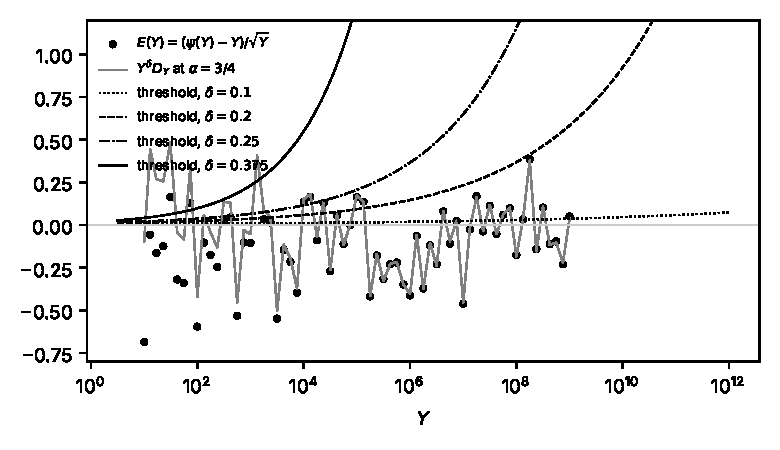
\includegraphics[width=\textwidth]{fig/v3/bo_cancel.pdf}
\caption{The normalised prime number theorem error $E(Y)$ at the checkpoints, the scaled truncation error $Y^\delta D_Y$ at $\alpha=\frac34$, which lies on top of it, and the thresholds $\frac{\xi'}{\xi}(\frac12+\delta)\,Y^\delta$ of~\eqref{bo:eq:cert}. The certificate at level $\frac12+\delta$ fails while $E$ can still reach the threshold.}
\label{bo:fig:cancel}
\end{figure}

\subsection{Away from the origin: a sharp cutoff band limits each zero}

For $t\ne0$ the truncated arithmetic block has an exact description in terms of the zeros, and it shows what a finite set of primes can and cannot see. Let $L=\log Y$, and define the truncated density by $\pi u_{\alpha,Y}(t)=\Re[G(s)-F_Y(s)]=B_\alpha(t)+G(\alpha)-\Re F_Y(\alpha+it)$.

\begin{theorem}[Sharp cutoff]\label{bo:thm:sharpcut}
Let $Y>1$ not be a prime power and $s=\alpha+it$ not a zero of $\zeta$ or the point $1$. Then, with no hypothesis on $\alpha$ or on the zeros,
\[
F_Y(s)=F(s)+\sum_\rho\frac{e^{-(s-\rho)L}}{s-\rho}+\sum_{k\ge1}\frac{e^{-(s+2k)L}}{s+2k},
\]
the sum over zeros in symmetric order, and therefore
\begin{equation}\label{bo:eq:sharp}
\pi\,u_{\alpha,Y}(t)=\sum_\rho\Re\,\frac{1-e^{-(s-\rho)L}}{s-\rho}\;-\;\Re\sum_{k\ge1}\frac{Y^{-(s+2k)}}{s+2k}.
\end{equation}
If the zero is $\rho=\frac12+i\gamma$ on the critical line, its term is
\begin{align*}
k_{\delta,L}(x)&=\int_0^{L}e^{-\delta w}\cos(xw)\dd w\\
&=\frac{\delta\bigl(1-Y^{-\delta}\cos xL\bigr)+x\,Y^{-\delta}\sin xL}{\delta^2+x^2},\qquad x=t-\gamma .
\end{align*}
\end{theorem}

\begin{proof}
The proof is Perron's formula at fixed $Y$. The only limits are $T\to\infty$ and a shift of the contour to the left.

(a) For $c>0$, $y>0$, $y\ne1$ and $T>0$, $|\frac1{2\pi i}\int_{c-iT}^{c+iT}y^w\frac{\dd w}w-\mathbf 1_{y>1}|\le y^c\min(1,\frac1{\pi T|\log y|})$ (Davenport~\cite{Davenport}, Chapter 17). Take $c=2+|\Re s|$, $y=Y/n$, multiply by $\Lambda(n)n^{-s}$ and sum over $n$. The series $\sum\Lambda(n)n^{-\Re s-c}$ converges, so the sum may be exchanged with the finite integral, and with $\eta_Y=\min_{\Lambda(n)\ne0}|\log(Y/n)|>0$ (this is the only use of the assumption that $Y$ is not a prime power)
\[
\Bigl|\sum_{n<Y}\Lambda(n)n^{-s}-\frac1{2\pi i}\int_{c-iT}^{c+iT}\Bigl(-\frac{\zeta'}{\zeta}\Bigr)(s+w)Y^w\frac{\dd w}w\Bigr|\le\frac{Y^c\,|\zeta'/\zeta(\Re s+c)|}{\pi T\eta_Y}.
\]

(b) Choose $T_j\to\infty$ with $|t\pm T_j-\gamma|\ge1/(C\log T_j)$ for every ordinate. The classical bounds for $\zeta'/\zeta$ (Davenport~\cite{Davenport}, Chapter 17) make the horizontal sides of the rectangle with vertical sides $\Re w=c$ and $\Re(s+w)=-2m-1$ tend to $0$ as $j\to\infty$, and the left side tend to $0$ as $m\to\infty$ with $j$ fixed. The residues of $(-\frac{\zeta'}{\zeta})(s+w)Y^w/w$ are $-\frac{\zeta'}{\zeta}(s)$ at $w=0$, $\frac{Y^{1-s}}{1-s}$ at $w=1-s$, $-\frac{Y^{\rho-s}}{\rho-s}$ at each zero, and $\frac{Y^{-2k-s}}{s+2k}$ at $w=-2k-s$. Hence
\[
\sum_{n\le Y}\Lambda(n)n^{-s}=-\frac{\zeta'}{\zeta}(s)+\frac{Y^{1-s}}{1-s}+\lim_{T}\sum_{|\gamma|<T}\frac{Y^{\rho-s}}{s-\rho}+\sum_{k\ge1}\frac{Y^{-2k-s}}{s+2k}.
\]
The zeros with $T-|t|\le|\gamma|\le T+|t|$ contribute $O((1+|t|)Y^{1-\Re s}\log T/T)$, so the limit exists in symmetric order.

(c) Subtract $\int_1^Yy^{-s}\dd y=\frac{Y^{1-s}-1}{1-s}$ and use $F=-\frac{\zeta'}{\zeta}-\frac1{s-1}$. This is the first formula. Then $G-F_Y=(G-F)-(F_Y-F)$ and~\eqref{bo:eq:xi} give~\eqref{bo:eq:sharp}. The closed form of the kernel is the elementary integral.
\end{proof}

The order of the limits matters. The classical form of the explicit formula with error $O(y\log^2(yT)/T)$ may not be integrated against $y^{-\alpha-1}$ over an infinite range when $\alpha<1$, because that integral diverges. In the proof above no integral beyond $Y$ occurs and the prime side is a finite sum: $T\to\infty$ at fixed $Y$, and only afterwards $Y\to\infty$.

The Cauchy kernel of a zero is $\delta/(\delta^2+x^2)=\int_0^\infty e^{-\delta w}\cos(xw)\dd w$. The theorem says that using the primes up to $Y$ cuts this Fourier integral off at the frequency $\log Y$, zero by zero.

\begin{corollary}[Window of positivity]\label{bo:cor:window}
$k_{\delta,L}(x)\ge0$ whenever $|x|\le\delta\,(Y^{\delta}-1)$. Outside this window the kernel is oscillating, with period $2\pi/L$ and envelope $Y^{-\delta}/|x|$ for large $|x|$.
\end{corollary}

\begin{proof}
The numerator is at least $\delta(1-Y^{-\delta})-|x|Y^{-\delta}$.
\end{proof}

The window is sufficient, not necessary, and the sign changes begin near $|x|\approx\delta Y^\delta$. The primes up to $Y$ show each zero as a positive peak within distance about $\delta Y^\delta$ of its ordinate. Farther away the zero contributes a sign changing tail that decays only like $1/|x|$, and the tails of all the zeros add up to the Chebyshev error. At the origin the nearest zeros are at $\pm14.13$, and the window of that one zero reaches the origin when $\delta(Y^\delta-1)\ge14.13$. This is a statement about one kernel. It does not decide the sign of the total truncated density, which is what Remark~\ref{bo:comp:ledger} measured, and the closeness of $13$ to $14.13$ should not be read as an explanation.

\begin{remark}[Computation]\label{bo:comp:sharp}
With the prime powers to $10^7$ and the first $6703$ zeros, the two sides of~\eqref{bo:eq:sharp} agree on $0\le t\le60$ to within $6\times10^{-4}$ at $\alpha=\frac34$ and $4\times10^{-4}$ at $\alpha=\frac78$, for $Y=10^2,\dots,10^7$; the difference is the omitted tail of the zeros. At $\alpha=\frac34$ the truncated density is negative on $20$, $4.6$, $4.2$, $0$, $1.0$ and $0$ per cent of $[0,60]$ for $Y=10^2$ to $10^7$: positivity is not monotone in the cutoff. At $\alpha=\frac78$ it is negative on $8$ per cent at $Y=10^2$ and nowhere from $Y=10^3$ on (Figure~\ref{bo:fig:bandlimit}). % UNVERIFIED: not rerun in the W4 verification
\end{remark}

\begin{figure}[ht]
\centering
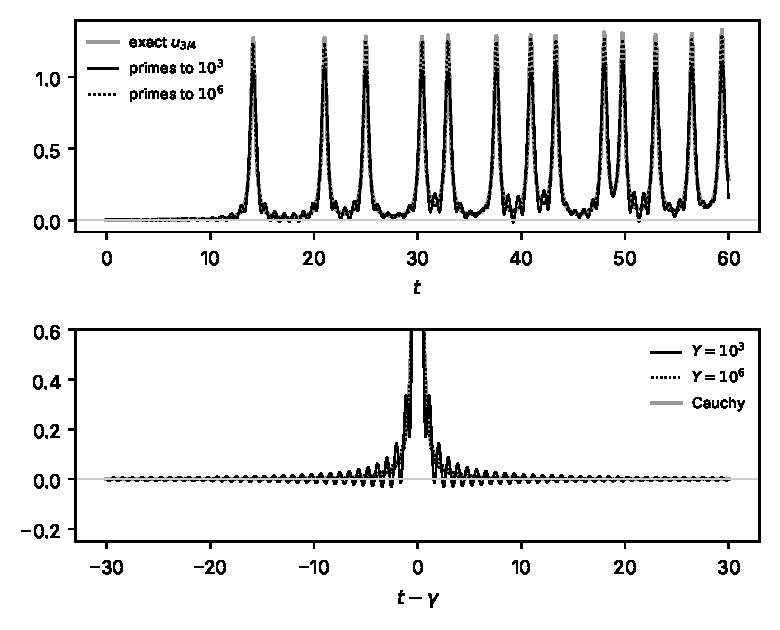
\includegraphics[width=\textwidth]{fig/v3/bo_bandlimit.pdf}
\caption{Above: $u_{3/4}$ and its truncations to the primes below $10^3$ and $10^6$. Below: the band limited kernel $k_{\delta,L}$ of one zero at $\delta=\frac14$, against the Cauchy kernel.}
\label{bo:fig:bandlimit}
\end{figure}

\section{Fej\'er weights: every zero pays positively}\label{bo:sec:fejerledger}

The sign changes of $k_{\delta,L}$ come from the sharp edge of the cutoff. Replace it by the triangular weight $(1-\log y/L)_+$. Put
\[
F^C_L(s)=\int_{[1,Y]}\Bigl(1-\frac{\log y}L\Bigr)y^{-s}\dd R(y)=\sum_{n\le Y}\Lambda(n)\Bigl(1-\frac{\log n}L\Bigr)n^{-s}-\kappa_L(s-1),
\]
with the entire kernel
\[
\kappa_L(z)=\int_0^L\Bigl(1-\frac wL\Bigr)e^{-zw}\dd w=\frac1z-\frac{1-e^{-zL}}{Lz^2},\qquad T_L(s)=\frac1L\sum_{k\ge1}\frac{1-e^{-(s+2k)L}}{(s+2k)^2}.
\]
Then $\pi u^C_{\alpha,L}(t)=\Re[G(s)-F^C_L(s)]$ is the Ces\`aro truncated density. The weight is the average over $v\in(0,L)$ of the sharp truncations at $e^v$: $F^C_L=\frac1L\int_0^LF_{e^v}\dd v$ by Fubini on a finite interval.

\begin{theorem}[Fej\'er ledger]\label{bo:thm:cesaro}
For every $L>0$ (no condition on $Y=e^L$) and every complex $s$ not a zero of $\zeta$ or $-2k$,
\begin{equation}\label{bo:eq:fejerid}
G(s)-F^C_L(s)=\sum_\rho\kappa_L(s-\rho)-T_L(s),
\end{equation}
where $\sum_\rho\kappa_L(s-\rho)$ means $\frac{\xi'}{\xi}(s)-\sum_\rho\frac{1-e^{-(s-\rho)L}}{L(s-\rho)^2}$, an absolutely convergent second series. Taking real parts,
\begin{equation}\label{bo:eq:fejerre}
\pi\,u^C_{\alpha,L}(t)=\sum_\rho\Re\,\kappa_L(s-\rho)-\Re\,T_L(s),
\end{equation}
and every term of the zero sum is nonnegative whenever $\Re(s-\rho)=\alpha-\beta\ge0$:
\[
\Re\,\kappa_L(a+ix)=\int_0^L\Bigl(1-\frac wL\Bigr)e^{-aw}\cos(xw)\dd w\ \ge0\qquad(a\ge0,\ x\in\mathbb R),
\]
strictly if $a>0$, and $\Re\kappa_L(ix)=(1-\cos xL)/(Lx^2)$.
\end{theorem}

\begin{proof}
(a) For $c>0$ and $y>0$, $\frac1{2\pi i}\int_{(c)}y^w\frac{\dd w}{w^2}=\log^+y$, absolutely convergent. With $c=2+|\Re s|$ and Fubini, $\frac1{2\pi i}\int_{(c)}(-\frac{\zeta'}{\zeta})(s+w)Y^w\frac{\dd w}{w^2}=\sum_{n\le Y}\Lambda(n)n^{-s}\log\frac Yn$.

(b) Shift the line to the left as in Theorem~\ref{bo:thm:sharpcut}. With $w^{-2}$ in place of $w^{-1}$ the horizontal sides are $O(Y^c\log^2T_j/T_j^2)$, the left side tends to $0$, and the residue series converge absolutely, so no ordering issue arises. The residues are: at $w=0$ (a double pole) $-(\frac{\zeta'}{\zeta})'(s)-L\frac{\zeta'}{\zeta}(s)$; at $w=1-s$, $\frac{Y^{1-s}}{(1-s)^2}$; at $w=\rho-s$, $-\frac{Y^{\rho-s}}{(\rho-s)^2}$; at $w=-2k-s$, $-\frac{Y^{-2k-s}}{(s+2k)^2}$. Subtract $\int_1^Y\log\frac Yy\,y^{-s}\dd y$:
\[
L\,F^C_L(s)=L\,F(s)+F'(s)-\sum_\rho\frac{e^{-(s-\rho)L}}{(s-\rho)^2}-\sum_{k\ge1}\frac{e^{-(s+2k)L}}{(s+2k)^2}.
\]

(c) By~\eqref{bo:eq:xi}, $F=G-\sum_\rho(s-\rho)^{-1}$ and $F'=G'+\sum_\rho(s-\rho)^{-2}$, and $G'(s)=\frac14\psi'(1+\frac s2)=\sum_{k\ge1}(s+2k)^{-2}$. Insert these and divide by $L$: this is~\eqref{bo:eq:fejerid}.

(d) For the sign, $h(w)=(1-|w|/L)_+e^{-a|w|}$ has Fourier transform $2\Re\kappa_L(a+ix)$, and $\hat h$ is $\frac1{2\pi}$ times the convolution of $L\,\mathrm{sinc}^2(\frac{\cdot L}2)\ge0$ with $2a/(a^2+x^2)>0$. For $a=0$ the transform is the Fej\'er kernel.
\end{proof}

For $a<0$ the kernel is not positive: $\Re\kappa_{20}(-0.05+0.2777i)=-1.63$. So a zero to the right of the level always carries some negative Fej\'er kernels.

\begin{corollary}\label{bo:cor:fejersmooth}
(1) If $\alpha\ge\Theta$ then every zero kernel in~\eqref{bo:eq:fejerre} is nonnegative at every height, so $\pi u^C_{\alpha,L}(t)\ge-\Re T_L(s)\ge-\psi'(1+\frac\alpha2)/(2L)$ for all $t$ and $L$. In particular this holds for all $\alpha\ge\frac12$ under RH. (2) If $\alpha>\Theta$, then $\sum_\rho\Re\kappa_L(s-\rho)=(\Phi_L*\pi u_\alpha)(t)$, with the Fej\'er kernel $\Phi_L(\xi)=\frac L{2\pi}(\frac{\sin(L\xi/2)}{L\xi/2})^2$: the triangular weight in $\log y$ is exactly Fej\'er smoothing in $t$. (3) If $\alpha\ge\Theta$ then $\pi u^C_{\alpha,L}(t)\to\pi u_\alpha(t)$ as $L\to\infty$ with error $O_{\alpha,t}(1/L)$, because the difference is $\sum_\rho\frac{1-e^{-(s-\rho)L}}{L(s-\rho)^2}$ plus $T_L$, and $|e^{-(s-\rho)L}|\le1$ for both members of each pair $(\rho,1-\bar\rho)$. For $\alpha<\Theta$ the Fej\'er means diverge exponentially in $L$.
\end{corollary}

With Fej\'er weights on the primes and on the pole, the cancellation becomes one signed: every zero at or to the left of the level contributes a nonnegative kernel at every height and every cutoff. The only negative entry in the whole ledger is the trivial zero term $-\Re T_L(s)$. It is explicit and archimedean: for large $L$ it is $-\frac1{4L}\Re\psi'(1+\frac s2)$, of size $0.2993/L$ at the origin when $\alpha=\frac12$, and decaying like $1/t^2$ in the height. The sign of the trivial term is not definite for finite $L$ at arbitrary $t$ (it reverses at $\alpha=0.75$, $L=0.1$, $t=\pi/L$), so the statement above is a statement for large $L$. Positivity of the Fej\'er truncation is then a race between the zeros and one digamma term.

\subsection{The Fej\'er threshold at the origin}

At $t=0$ put $\Phi_\delta(L)=L\,\pi u^C_{\alpha,L}(0)=LG(\alpha)-\sum_{n\le e^L}\Lambda(n)n^{-\alpha}\log\frac{e^L}n+\int_1^{e^L}\log\frac{e^L}y\,y^{-\alpha}\dd y$, and $L^*(\delta)=\sup\{L>0:\Phi_\delta(L)<0\}$. Write $X_1=\frac{\xi'}{\xi}(\alpha)$, $X_2=(\frac{\xi'}{\xi})'(\alpha)$, $P=\frac14\psi'(1+\frac\alpha2)$ and $\tau(L)=\sum_{k\ge1}e^{-(\alpha+2k)L}/(\alpha+2k)^2\in(0,Pe^{-(\alpha+2)L}]$. Let
\[
K=\frac{\psi'(5/4)}{4q}=6.4776537074,
\]
and let $c_\pm$ be the positive roots of $c+1\mp e^{-c}=K$, so that $c_+=5.4818154746$ and $c_-=5.4734570084$, and $K-1=5.4776537074$ lies between them.

\begin{theorem}[Threshold at the origin]\label{bo:thm:threshold}
Let $0<\delta<\frac12$ and $\alpha=\frac12+\delta$.
\begin{enumerate}
\item (Proved.) $\Phi_\delta(L)=LX_1+X_2-P+\tau(L)+\sum_\rho\Re\frac{e^{-(\alpha-\rho)L}}{(\alpha-\rho)^2}$.
\item (Proved, unconditional.) $L^*(\delta)<\infty$ if and only if $\Theta\le\frac12+\delta$. Hence RH holds if and only if $L^*(\delta)<\infty$ for every $\delta>0$. For $L<\log2$ there are no prime powers and $\Phi_\delta(L)<0$.
\item (Proved under RH, effective.) $\bigl|\Phi_\delta(L)-(LX_1+X_2-P)-\tau(L)\bigr|\le e^{-\delta L}X_1/\delta$. Let $L_\pm(\delta)$ be the unique positive roots of $LX_1+X_2-P\mp e^{-\delta L}X_1/\delta$. Then $\Phi_\delta>0$ on $(L_+,\infty)$ and $\Phi_\delta<0$ on $(0,L_1)$ with $0<L_--L_1\le\frac{Pe^{-(\alpha+2)L_1}}{X_1(1-e^{-\delta L_1})}$, so $L_1\le L^*\le L_+$ and $\delta L_\pm(\delta)\to c_\pm$.
\item (Proved under RH.) $\delta L^*(\delta)\to c_+=5.4818154746$ as $\delta\to0+$. The lower bound for $\liminf$ is not effective.
\item (Proved under RH.) Uniformly for $L>0$ and $0<\delta\le\frac14$, with $S(L)=\sum_\rho\frac{\cos\gamma L}{\gamma^2}$ (uniformly almost periodic, $S(0)=q$, $|S|\le q$, mean $0$),
\[
\Phi_\delta(L)=q(\delta L+1)-\tfrac14\psi'(\tfrac54)-e^{-\delta L}S(L)+\tau(L)+O(\delta+\delta^3L).
\]
So at fixed $c=\delta L$, $\Phi_\delta(c/\delta)=e^{-c}[\theta(c)-S(c/\delta)]+O(\delta)$ with $\theta(c)=q(c+1-K)e^c$ increasing. All three terms are $O(1)$.
\item (Proved under RH.) For every $[a,b]\subset(c_*,c_+)$, where $\theta(c_*)=\inf S$, the number of sign changes of $\Phi_\delta$ on $[a/\delta,b/\delta]$ is at least $C_{a,b}/\delta$ for $\delta<\delta_0(a,b)$. From the zeros, $c_*\le5.47531$, and under linear independence of the ordinates $\inf S=-q$ and $c_*=c_-$. For $c\le c_--\varepsilon$ one has $\Phi_\delta<0$, and for $c\ge c_++\varepsilon$, $\Phi_\delta>0$.
\end{enumerate}
\end{theorem}

\begin{proof}
(1) Multiply~\eqref{bo:eq:fejerid} at $s=\alpha$ by $L$. Then $L\sum_\rho\kappa_L(\alpha-\rho)=LX_1+X_2+\sum_\rho\frac{e^{-(\alpha-\rho)L}}{(\alpha-\rho)^2}$, because $\sum_\rho(\alpha-\rho)^{-1}=X_1$ and $-\sum_\rho(\alpha-\rho)^{-2}=X_2$, and $-LT_L(\alpha)=-P+\tau(L)$.

(2) For $\Re z>1$, Fubini and $\int_{\log y}^\infty(L-\log y)e^{-zL}\dd L=y^{-z}/z^2$ give $\int_0^\infty\Phi_\delta(L)e^{-zL}\dd L=\frac{G(\alpha)-F(\alpha+z)}{z^2}$. If $\Phi_\delta\ge0$ on $[L_0,\infty)$, Landau's theorem (Widder~\cite{Widder41}, Chapter II, Theorem 5b) says that the abscissa of convergence, if finite, is a singular point of the function represented. That function differs from $\frac{G(\alpha)-F(\alpha+z)}{z^2}$ by an entire function, and it is analytic at every real $z>0$, since $F(\sigma)$ is analytic for real $\sigma>\frac12$ ($\zeta(\sigma)\ne0$ on $(0,1)$ because $(1-2^{1-\sigma})\zeta(\sigma)=\sum(-1)^{n-1}n^{-\sigma}>0$, and $F$ is regular at $1$). So the integral converges on $\Re z>0$, $F(\alpha+z)$ is analytic there, and $\zeta$ has no zero with $\beta>\alpha$. Conversely, if $\Theta\le\alpha$ then $|e^{-(\alpha-\rho)L}|\le1$ for both members of every pair and (1) gives $\Phi_\delta(L)\ge LX_1+X_2-P-\sum_\rho|\alpha-\rho|^{-2}\to\infty$. For $0<L<\log2$, $\Phi_\delta(L)=LG(\alpha)+\frac{e^{(1-\alpha)L}-1-(1-\alpha)L}{(1-\alpha)^2}\le LG(\alpha)+0.71L^2<0$, since $G(\alpha)\le G(1)=-0.5543$.

(3) Under RH, $\alpha-\rho=\delta-i\gamma$ and $\sum_\rho(\delta^2+\gamma^2)^{-1}=X_1/\delta$, which gives the bound. The functions $g_\pm(L)=LX_1+X_2-P\mp e^{-\delta L}X_1/\delta$ have $g_\pm'=X_1(1\pm e^{-\delta L})>0$, $g_\pm(0)<2q-P<0$ (under RH $X_1/\delta<q$, $X_2<q$, and $P\ge\frac14\psi'(\frac32)=0.2337$) and $g_\pm\to\infty$, so the roots are unique, and $\Phi_\delta\ge g_++\tau>0$ beyond $L_+$. For $L\ge\log2$, $\Phi_\delta\le g_-(L)+Pe^{-(\alpha+2)L}$. This sum is negative at $\log2$ (at most $q\log2/2+2q-0.82P<-0.08$, since $2^{-(\alpha+2)}<0.18$), and its derivative $X_1(1-e^{-\delta L})-(\alpha+2)Pe^{-(\alpha+2)L}$ is increasing, so it changes sign at most once, from negative to positive, and it is positive at $L_-$. It is therefore negative exactly on $[\log2,L_1)$ for a unique $L_1<L_-$, and the mean value theorem bounds $L_--L_1$. In the variable $c=\delta L$ the root equations read $c\frac{X_1}\delta+X_2-P\mp e^{-c}\frac{X_1}\delta=0$ with $X_1/\delta\to q$, $X_2\to q$, $P\to Kq$. The limit equations $q(c+1-K\mp e^{-c})=0$ have simple roots $c_\pm$, and the implicit function theorem applies.

(5) $X_1=q\delta+O(\delta^3)$ by oddness, $X_2=q+O(\delta^2)$ and $P=\frac14\psi'(\frac54)+O(\delta)$. With $T(\delta,L)=\sum_\rho\Re\frac{e^{i\gamma L}}{(\delta-i\gamma)^2}$ one has $\sum_\rho\Re\frac{e^{-(\alpha-\rho)L}}{(\alpha-\rho)^2}=e^{-\delta L}T$ and $|T+S|\le\delta\sum_\rho(2|\gamma|^{-3}+\delta\gamma^{-4})=O(\delta)$ uniformly in $L$.

(4) The upper bound is (3). For the lower bound fix $\varepsilon\in(0,1)$ and $\eta=\varepsilon/4$. By Bohr's theorem the set of $\eta q$ almost periods of $S$ is relatively dense with inclusion length $\ell$, and $S(\tau)>q(1-\eta)$ on it. For $\delta\le\varepsilon/(2\ell)$ the window $[(c_+-\varepsilon)/\delta,(c_+-\varepsilon/2)/\delta]$ contains an almost period $L$. By (5), $\Phi_\delta(L)\le q[h(c)+\eta e^{-c}]+O(\delta)$ with $h(c)=c+1-e^{-c}-K$, $h(c_+)=0$, $h'\ge1$, so $\Phi_\delta(L)\le-q\varepsilon/4+O(\delta)<0$ and $L^*\ge(c_+-\varepsilon)/\delta$.

(6) By (5), $\Phi_\delta<0$ where $S>\theta(\delta L)+C\delta$ and $\Phi_\delta>0$ where $S<\theta(\delta L)-C\delta$. On $[a,b]$, $\theta\in[\theta(a),\theta(b)]$ with $\theta(b)<q$ and $\theta(a)>\inf S$. The sets $\{S>(\theta(b)+q)/2\}$ and $\{S<\theta(a)-\eta'\}$ are both relatively dense, being unions of translates by almost periods, so they alternate at least $\frac{b-a}{2\delta\ell'}-2$ times in $[a/\delta,b/\delta]$. For $c\le c_--\varepsilon$ and $c\ge c_++\varepsilon$ use (3).
\end{proof}

The three constants differ only at order $e^{-c}\approx0.0042$. The constant $c_-$ is where the permanent failure ends, $K-1$ is where the $L$ average of $\Phi_\delta$ vanishes (it corresponds to $S$ at its mean $0$), and $c_+$ is the last failure (it corresponds to $S$ near its supremum $q$). If the oscillating term $e^{-\delta L}S(L)$ were dropped one would obtain $K-1$ as the limit of $\delta L^*$. It is of leading order and cannot be dropped.

\begin{remark}[Computation]\label{bo:comp:cesaro}
With the zero table of $8000$ ordinates (to $8148.19$) and the smooth tail, Table~\ref{bo:tab:cesaro} gives $L^*$ from the zeros, and Table~\ref{bo:tab:transition} the bracket of part (3) and the number of sign changes in $[L_-,L_+]$. Each scan has step $10^{-3}$ in $L$ followed by bisection, and the tail beyond the $8000$th zero changes $\Phi$ by at most $1.3\times10^{-6}$. At $\delta\le0.005$ there is more than one sign change: $5$, $7$, $17$, $33$, $67$, $131$ at $\delta=0.005,0.002,0.001,0.0005,0.0002,0.0001$, growing like $1/\delta$. At $\alpha=0.75$ and $0.875$ the Fej\'er prime side (all prime powers to $10^8$) agrees with the zero side to $2\times10^{-4}$, which validates the kernel $\kappa_L$ and the trivial term. At $\alpha=\frac78$ the Fej\'er density is positive on $[0,60]$ from $Y=10^6$ on, and at $\alpha=\frac34$ it is still negative at the origin at $Y=10^7$; the minimum over $t$ is at the origin in every case tried. % UNVERIFIED: the statements at alpha = 7/8 and 3/4 at Y = 10^6, 10^7 are from the draft
\end{remark}

\begin{table}[ht]
\centering\small
\begin{tabular}{@{}lccccccc@{}}
\toprule
$\delta$ & $0.375$ & $0.25$ & $0.2$ & $0.15$ & $0.1$ & $0.05$ & $0.02$\\
\midrule
$L^*$ & $11.621$ & $18.744$ & $24.139$ & $33.193$ & $51.352$ & $106.041$ & $270.343$\\
$\delta L^*$ & $4.358$ & $4.686$ & $4.828$ & $4.979$ & $5.135$ & $5.302$ & $5.407$\\
$\log_{10}Y^*$ & $5.05$ & $8.14$ & $10.48$ & $14.42$ & $22.30$ & $46.05$ & $117.41$\\
\bottomrule
\end{tabular}
\caption{The Fej\'er cutoff $Y^*=e^{L^*}$ needed for the primes to show positivity at the origin, from the zeros (computed). The values of $\delta L^*$ increase towards $c_+=5.4818$.}
\label{bo:tab:cesaro}
\end{table}

\begin{table}[ht]
\centering\small
\begin{tabular}{@{}lcccc@{}}
\toprule
$\delta$ & $\delta L_-$ & $\delta L^*$ & $\delta L_+$ & sign changes in $[L_-,L_+]$\\
\midrule
$0.05$ & $5.29769$ & $5.30205$ & $5.30765$ & $1$\\
$0.02$ & $5.40207$ & $5.40686$ & $5.41104$ & $1$\\
$0.01$ & $5.43758$ & $5.44215$ & $5.44624$ & $1$\\
$0.005$ & $5.45547$ & $5.46054$ & $5.46398$ & $5$\\
$0.002$ & $5.46625$ & $5.47208$ & $5.47467$ & $7$\\
$0.001$ & $5.46985$ & $5.47560$ & $5.47824$ & $17$\\
$0.0005$ & $5.47165$ & $5.47782$ & $5.48003$ & $33$\\
$0.0002$ & $5.47274$ & $5.47864$ & $5.48110$ & $67$\\
$0.0001$ & $5.47310$ & $5.47899$ & $5.48146$ & $131$\\
limit & $c_-=5.47346$ & $c_+=5.48182$ & $c_+=5.48182$ & $\asymp1/\delta$\\
\bottomrule
\end{tabular}
\caption{The effective bracket of Theorem~\ref{bo:thm:threshold}(3) and the transition region (computed from $8000$ zeros). After removing the drift $-3.6\,\delta$ the sign changes at $\delta=10^{-3}$ lie in $[5.476,5.480]$.}
\label{bo:tab:transition}
\end{table}

The convergence $\delta L^*(\delta)\to c_+$ is extremely slow. On $1\le L\le3000$ the largest value of $S/q$ is $0.567$, and $S$ approaches $q$ only at simultaneous near alignments of many ordinates, which Dirichlet's theorem places at astronomically large $L$. At every accessible $\delta$ the observed $\delta L^*$ sits near the $c$ for which $\theta(c)$ equals the largest value of $S$ that has been attained, strictly inside $[c_-,c_+]$. The honest statement is the rigorous bracket of part (3) together with the limit of part (4). For comparison, the Fej\'er cutoff $e^{5.48/\delta}$ exceeds the empirical sharp rule $(13/\delta)^{1/\delta}$ for $\delta>0.054$ and is smaller below.

\subsection{The Fej\'er criterion at any height}\label{bo:sec:fejer}

Theorem~\ref{bo:thm:cesaro} is an identity at every level. Read at one point, it becomes a criterion. For $\alpha\ge\frac12$, $Y>1$, $L=\log Y$ and real $t$ put
\[
S_L(\alpha,t)=\sum_\rho\Re\,\kappa_L(\alpha+it-\rho)=\Re\bigl[G(s)-F^C_L(s)+T_L(s)\bigr].
\]
At $t=0$ this is
\begin{multline*}
S_\alpha(Y)=G(\alpha)+\int_0^L\Bigl(1-\frac wL\Bigr)e^{(1-\alpha)w}\dd w+\frac1L\sum_{k\ge1}\frac{1-Y^{-(\alpha+2k)}}{(\alpha+2k)^2}\\
-\sum_{n\le Y}\Lambda(n)\Bigl(1-\frac{\log n}{\log Y}\Bigr)n^{-\alpha}.
\end{multline*}
The first three terms are explicit: the archimedean constant, the Fej\'er block of the pole, and the debt of the trivial zeros. The last is a finite sum over prime powers. For general $t$ the same expression is a finite prime sum plus elementary terms.

\begin{theorem}[Fej\'er criterion]\label{bo:thm:fejer}
Let $\alpha\ge\frac12$ and let $t$ be real such that no zero with $\beta>\alpha$ has ordinate $t$ or $-t$ (all $t$ outside a countable set, and always $t=0$). The following are equivalent:
\begin{enumerate}
\item $\xi$ has no zero in $\Re s>\alpha$, that is $\Theta\le\alpha$;
\item $S_L(\alpha,t)\ge0$ for all $L>0$;
\item $S_L(\alpha,t)\ge0$ for all $L\ge L_0$, for some $L_0$;
\item $S_L(\alpha,t)=O(e^{\varepsilon L})$ for every $\varepsilon>0$.
\end{enumerate}
In particular RH holds if and only if $S_\alpha(Y)\ge0$ for all large $Y$ at $\alpha=\frac12$, and under RH
\[
S_{1/2}(Y)=\frac2L\sum_{\gamma>0}\frac{2\sin^2(\gamma L/2)}{\gamma^2}.
\]
\end{theorem}

\begin{proof}
(1) implies (2) by Theorem~\ref{bo:thm:cesaro}, and (2) implies (3) trivially. For (3) or (4) implies (1), put $h(L)=L\,S_L(\alpha,t)$. From $L\kappa_L(z)=L/z-(1-e^{-zL})/z^2$ one has $|\Re L\kappa_L(z)|\le(L|\Re z|+1+e^{-L\Re z})/|z|^2$, summable over the zeros, so $|h(L)|\ll(1+L)^2e^{(\Theta-\alpha)^+L}$. For real $\lambda>\max(0,\Theta-\alpha)$, Fubini and $\int_0^\infty e^{-\lambda L}L\kappa_L(z)\dd L=\frac1{\lambda^2(\lambda+z)}$ give
\[
\int_0^\infty e^{-\lambda L}h(L)\dd L=\frac1{\lambda^2}\Re\frac{\xi'}{\xi}(\lambda+s)=\frac1{2\lambda^2}\Bigl[\frac{\xi'}{\xi}(\lambda+s)+\frac{\xi'}{\xi}(\lambda+\bar s)\Bigr].
\]
The right side is meromorphic with poles at $\lambda=0$ and at $\lambda=\rho-s$, $\rho-\bar s$. The residues of $\xi'/\xi$ are positive integers, so poles at the same point never cancel. Under (4) the integral converges absolutely for $\Re\lambda>0$, hence the right side is analytic there and every zero has $\beta\le\alpha$. Under (3), Landau's theorem says that the abscissa of convergence, if finite, is a real singularity of the right side. Its real singularities in $(0,\infty)$ would be points $\beta-\alpha$ with $\gamma=\pm t$, $\beta>\alpha$, which are excluded. So the abscissa is at most $0$ and $\Theta\le\alpha$. Finally (1) implies (4): every term is bounded by $(L|\Re z|+2)/|z|^2$, so $S_L=O(1)$ unless $t$ is the ordinate of a zero on the level, where $S_L=O(L)$. At $\alpha=\frac12$ under RH, $\Re\kappa_L(\mp i\gamma)=(1-\cos\gamma L)/(L\gamma^2)$, and the zeros come in pairs $\pm\gamma$.
\end{proof}

At $\alpha=\frac12$ and $t=0$ this is the oscillator criterion of Volume II, Proposition~\ref{yo:prop:tent} and Theorem~\ref{yo:thm:D}: $D=2f$ with $f(L)=L\,S_{1/2}(e^L)$ (Section~\ref{bo:sec:osc}), and the Landau argument is the one given there. The general form, with an arbitrary level and an arbitrary height, is what the ledger adds. The theorem is a member of the family of Weil's positivity criteria (Weil~\cite{Weil52}, Bombieri~\cite{Bombieri}), with Landau's theorem supplying the converse from a single test function at a single point. Under RH the slack is a $2\sin^2$ sum over the zeros: the kernel of the lemma on which these books are built appears on the dual side, with the roles of $\log n$ and $\gamma$ exchanged. Bondesson's blocks $1-\cos(t\log n)$ live on the primes with $t$ as the variable, and the slack $1-\cos(\gamma\log Y)$ lives on the zeros with $\log Y$ as the variable.

\paragraph{Weights.} A weight is a continuous $W:[0,1]\to\mathbb R$ with $W(0)=1$. It defines $F_{W,L}(s)=\int_{[1,Y]}W(\frac{\log y}L)y^{-s}\dd R(y)$ and the zero kernel $K_{W,L}(z)=\int_0^LW(u/L)e^{-zu}\dd u$, which is $\kappa_L$ for $W(u)=1-u$. Call $W$ \emph{admissible} if $\Re K_{W,L}(a+ix)\ge0$ for all $a\ge0$ and real $x$; then under RH the weighted ledger has a nonnegative kernel for every zero, every $\alpha\ge\frac12$ and every $t$.

\begin{proposition}[Admissible weights and the triangle]\label{bo:prop:triangle}
(a) $W$ is admissible if and only if its even extension $W_e(u)=W(|u|)1_{|u|\le1}$ is positive definite on $\mathbb R$. (b) For admissible $W$, $\int_0^1W\le\frac12$, with equality if and only if $W(u)=1-u$. Equivalently the triangle maximises the kernel at the origin $K_{W,L}(0)=L\int_0^1W$, uniquely. (c) The sharp cutoff $W\equiv1$ is not admissible, since $\Re K(ix)=\sin(xL)/x$. (d) The triangle is not optimal for the threshold: the defect $\frac1z-K_{W,L}(z)$ of the trivial zeros is of order $1/(Lz^2)$ for the triangle, but $O(L^{-2})$ for an admissible weight with $W'(0)=0$.
\end{proposition}

\begin{proof}
(a) At $a=0$, $2\Re K_{W,1}(ix)=\widehat{W_e}(x)$, and a continuous integrable function is positive definite if and only if its transform is nonnegative (Bochner). For $a>0$, $W_e(u)e^{-a|u|}$ is a product of positive definite functions, hence positive definite, with transform $2\Re K_{W,1}(a+ix)$. (b) The $1$ periodisation $\sum_kW_e(u+k)$ is continuous with Fourier coefficients $\widehat{W_e}(2\pi m)\ge0$ and value $W_e(0)=1$ at $0$ (because $W_e(\pm1)=0$). Nonnegative coefficients of a continuous function are summable with sum equal to that value, so $1\ge\widehat{W_e}(0)=2\int_0^1W$. Equality forces $\widehat{W_e}(2\pi m)=0$ for $m\ne0$; since $\widehat{W_e}\ge0$ has exponential type $\le1$, these zeros are double, so $\widehat{W_e}/(\frac{\sin(\xi/2)}{\xi/2})^2$ is entire of polynomial growth, hence an even polynomial $a+b\xi^2$, and integrability and $W_e(0)=1$ force $b=0$, $a=1$: the triangle. (c) is direct. (d) $1-W(v)=-W'(0^+)v+O(v^2)$ in $\frac1z-K_{W,L}(z)=\int_0^\infty(1-W_+(u/L))e^{-zu}\dd u$.
\end{proof}

The inequality in (b) is the one dimensional case of Tur\'an's extremal problem for positive definite functions (Siegel; Boas and Kac). So the triangle is optimal exactly in the Tur\'an sense, and the next section shows that a smoother admissible weight does better for the threshold. A convex decreasing weight $g$ with $g(0)=1$, $g(L)=0$ is a mixture of triangles, $g(w)=\int_0^L(1-w/a)_+\,\nu(\dd a)$ with $\nu(\dd a)=a\,g''(\dd a)$ a probability measure (Taylor's formula with integral remainder), so for every functional linear in the weight, $S^g_\alpha$ is an average of the values $S_\alpha(e^a)$, $0<a\le L$. In particular no convex weight certifies positivity at the origin at a smaller cutoff than the triangle does. % TODO for the authors: no bibliography entries for Siegel, Boas and Kac (Siegel32 is the wrong paper)

\begin{proposition}[Margin]\label{bo:prop:margin}
Assume RH.
\begin{enumerate}
\item On the line, $L\,S_{1/2}(e^L)=f(L)=\sum_{\gamma>0}2(1-\cos\gamma L)/\gamma^2$, and
\[
\liminf_{L\to\infty}f(L)=0,\qquad f(L)\le M=4\sum_{\gamma>0}\gamma^{-2}=0.0924199724617 .
\]
\item For $\alpha=\frac12+\delta$ with $\delta>0$, $S_\alpha(Y)=\frac{\xi'}{\xi}(\alpha)+O(1/L)\to\frac{\xi'}{\xi}(\alpha)>0$ as $Y\to\infty$.
\end{enumerate}
\end{proposition}

\begin{proof}
(1) The series converges uniformly, so $f$ is almost periodic in the sense of Bohr, and $f(0)=0$. For every $\varepsilon>0$ the $\varepsilon$ almost periods $\tau$ are relatively dense and $f(\tau)=|f(\tau)-f(0)|<\varepsilon$. So $f$ returns arbitrarily close to $0$ for arbitrarily large $L$. The upper bound is $1-\cos\le2$. (2) By Theorem~\ref{bo:thm:threshold}(1), $S_\alpha(Y)=X_1+(X_2+\sum_\rho\Re\frac{e^{-(\alpha-\rho)L}}{(\alpha-\rho)^2})/L$, and $|\cdot|\le X_2+\sum_\rho|\alpha-\rho|^{-2}$ is bounded.
\end{proof}

On the critical line the inequality that is equivalent to RH holds, if it holds, with no margin: the slack $f(L)/L$, already of size $1/L$, comes back arbitrarily close to $f=0$ infinitely often, at the cutoffs for which $\gamma L$ is nearly a multiple of $2\pi$ for all low zeros at once. No argument that proves $f\ge c$ with a fixed $c>0$ can be correct. Half a step above the line the picture is different: $S_\alpha(Y)$ tends to $\xi'/\xi(\alpha)\approx0.0462\,\delta$, the same linear margin as in Proposition~\ref{bo:prop:origin}.

\begin{remark}[Computation]\label{bo:comp:fejer}
With the prime powers to $10^7$ and $6000$ cutoffs from $3$ to $10^7$, the prime side $S_\alpha(Y)$ and the sum over the first $6703$ zeros, with a tail correction, agree to $1.5\times10^{-5}$ at $\alpha=\frac12$ and at $\alpha=\frac34$. % UNVERIFIED: agreement figure from the draft, not rerun
At $\alpha=\frac12$ the oscillator $f=L\,S_{1/2}(e^L)$ has mean $0.04620$ against $2\sum_{\gamma>0}\gamma^{-2}=0.04621$ (Figure~\ref{bo:fig:fejer}), and on $4\le L\le20.72$ (primes to $10^9$) it lies in $[0.02152,0.06890]$ (independent recomputation: minimum at $L=17.348$, maximum at $L=12.674$). From the zeros, out to $L=60$, its minimum is $0.02134$, at $L=25.38287$, that is $Y=1.056\times10^{11}$; this value is stable under the number of zeros ($300$ to $1500$) and its neglected tail has standard deviation about $10^{-5}$. The next minima are $0.0215$ (primes), $0.0245$ ($L=20.04$) and $0.0246$ ($L=34.70$). Primes to $1.06\times10^{11}$ have not been summed, so the value at $Y=10^{11}$ is a zero side value. Over $0\le t\le3000$ the Fej\'er density of Theorem~\ref{bo:thm:cesaro} has its minimum at $t=0$ in each of four cases tried, at the levels $\frac34$ and $\frac78$, and for $t\ge5$ it is at least $0.0138$. % UNVERIFIED: last sentence from the draft
\end{remark}

\begin{figure}[ht]
\centering
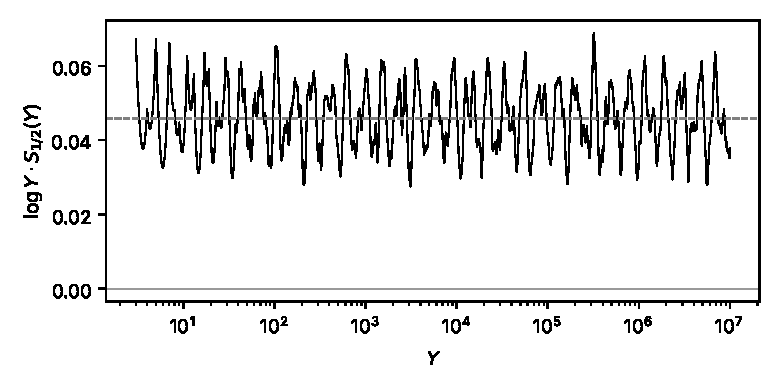
\includegraphics[width=\textwidth]{fig/v3/bo_fejer.pdf}
\caption{The slack of the Fej\'er criterion on the critical line, $f(L)=L\,S_{1/2}(e^L)$, computed from the primes. The dashed line is its mean $2\sum_{\gamma>0}\gamma^{-2}$. RH is the statement that the curve never goes below zero.}
\label{bo:fig:fejer}
\end{figure}

\section{A smooth window: a square root threshold}\label{bo:sec:smooth}

The Fej\'er window has a corner at the origin of the weight, $g'(0^+)=-1/L$, and this corner is what makes the trivial zero debt of order $1/L$ and the zero term $e^{-\delta L}S(L)/L$ of the same order. A weight that is flat at the origin does better. The window used here is the self convolution of a cosine lobe. Put $\omega=\pi/L$ and
\[
g_L(w)=\Bigl(1-\frac wL\Bigr)\cos\omega w+\frac1\pi\sin\omega w\quad(0\le w\le L),\qquad g_L=0\ (w>L).
\]
This is the classical test function in Weil's explicit formula approach to lower bounds for discriminants, usually credited to Poitou~\cite{Poitou77} (after Serre) and used by Odlyzko~\cite{Odlyzko90} and by Mestre, and in spectral analysis it is the Bohman window~\cite{Bohman61}. We have not found the threshold statement below, nor any threshold of order $\delta^{-1/2}$ for finite prime truncations of $\Re\xi'/\xi(\frac12+\delta)$, in the literature. % UNCHECKED: Poitou77 venue and year; attribution to Mestre has no entry in this volume (TODO for the authors)

\begin{lemma}[The window]\label{bo:lem:window}
Put $K_L(z)=\int_0^Lg_L(w)e^{-zw}\dd w$ and $D_L(z)=\frac1z-K_L(z)$.
\begin{enumerate}
\item $g_L(0)=1$, $g_L(L)=g_L'(0)=g_L'(L)=g_L''(L)=0$, $g_L''(0)=-\pi^2/L^2$, $g_L'(w)=-\omega(1-\frac wL)\sin\omega w\le0$, and $g_L$ is the normalised autocorrelation of $\cos(\pi x/L)1_{[-L/2,L/2]}$.
\item $K_L(z)=\frac z{z^2+\omega^2}+\frac{2\omega^2(1+e^{-zL})}{L(z^2+\omega^2)^2}$ is entire, and for real $a>0$, $D_L(a)=\frac1a\int_0^1\phi(u)e^{-aLu}\dd u$ with $\phi(u)=\pi(1-u)\sin\pi u\ge0$, $\int_0^1\phi=1$.
\item $\hat g_L(x)=\int g_L(|w|)e^{-ixw}\dd w=\frac{8\pi^2L\cos^2(xL/2)}{(\pi^2-x^2L^2)^2}\ge0$, so $\Re K_L(\delta+ix)\ge0$ for $\delta\ge0$, strictly for $\delta>0$.
\item For $\Re z\ge0$, $z\ne0$: $K_L(z)=\frac1z-\frac{\pi^2}{L^2z^3}+R_L(z)$ with $|R_L(z)|\le\frac A{L^3|z|^4}$, $A=4\pi^2+\int_0^1|\pi^4(1-u)\cos\pi u-3\pi^3\sin\pi u|\dd u=100.7304$.
\end{enumerate}
\end{lemma}

\begin{proof}
(1) and (2) are elementary integrals: $\int_0^L\cos(\omega w)e^{-zw}\dd w=\frac{(1+e^{-zL})z}{z^2+\omega^2}$ since $e^{\pm i\pi}=-1$, and the other two pieces follow by differentiation in $z$. For (3), the autocorrelation of $p_L=\cos(\omega x)1_{[-L/2,L/2]}$ is $\frac L2g_L(|w|)$, so $\hat g_L=\frac2L|\hat p_L|^2\ge0$, and $\Re K_L(\delta+ix)=\frac1{2\pi}\int\hat g_L(y)\frac{\delta\,\dd y}{\delta^2+(x-y)^2}$. For (4) integrate by parts four times; the boundary terms of orders $z^{-1}$ to $z^{-3}$ follow from (1), and $|e^{-zw}|\le1$, $L^3\int_0^L|g_L''''|=\int_0^1|L^4g_L''''(Lu)|\dd u$ with $L^4g_L''''(Lu)=\pi^4(1-u)\cos\pi u-3\pi^3\sin\pi u$.
\end{proof}

\begin{proposition}[Smooth Fej\'er ledger]\label{bo:prop:smoothid}
Let $F^g_L(s)=\int_{[1,e^L]}g_L(\log y)y^{-s}\dd R(y)=\sum_{n\le e^L}\Lambda(n)g_L(\log n)n^{-s}-K_L(s-1)$. For every $L>0$ and every $s$ that is not a zero of $\zeta$ or $-2k$, with no hypothesis on the zeros,
\[
G(s)-F^g_L(s)=\frac{\xi'}{\xi}(s)-\sum_\rho D_L(s-\rho)-\sum_{k\ge1}D_L(s+2k),
\]
both series converging absolutely. At $s=\alpha$, $C^g_\delta(L)=G(\alpha)-F^g_L(\alpha)=\frac{\xi'}{\xi}(\alpha)-Z_\delta(L)-T_\alpha(L)$ with $Z_\delta(L)=\sum_\rho\Re D_L(\alpha-\rho)$ and $T_\alpha(L)=\sum_kD_L(\alpha+2k)$. The function $C^g_\delta$ is $C^2$ in $L$, since a prime power enters with weight vanishing to second order.
\end{proposition}

\begin{proof}
Since $g_L(L)=g_L'(L)=0$, $g_L(w)=\int_0^L(1-\frac wv)_+\,v\,g_L''(v)\dd v$, and $\int_0^Lvg_L''(v)\dd v=1$. Integrate the Fej\'er identity~\eqref{bo:eq:fejerid} with $L$ replaced by $v$ against $v\,g_L''(v)\dd v$ on $[0,L]$. The left side becomes $G-F^g_L$ (Fubini on a finite sum and a bounded integral). The zero terms become $\int_0^L\frac{1-e^{-zv}}{vz^2}\,vg_L''(v)\dd v=-z^{-2}\int_0^Le^{-zv}g_L''(v)\dd v=D_L(z)$, using $\int_0^Lg_L''=0$; Fubini is justified by $\sum_\rho|s-\rho|^{-2}<\infty$ and the bound $|z|^{-2}(1+e^{L\max(0,-\Re z)})|g_L''(v)|$, so no hypothesis on the zeros is used. The trivial terms are treated the same way.
\end{proof}

\begin{proposition}[The two remainders]\label{bo:prop:remainders}
(a) The function
\[
T_\alpha(L)=\sum_k\frac1{\alpha+2k}\int_0^1\phi(u)e^{-(\alpha+2k)Lu}\dd u>0
\]
is strictly decreasing in $L$, tends to $+\infty$ as $L\to0+$ and to $0$ as $L\to\infty$, and
\[
T_\alpha(L)=\frac{\pi^2B_3(\alpha)}{L^2}-\frac{2\pi^2B_4(\alpha)}{L^3}+O(L^{-4}),\qquad B_j(\alpha)=\sum_{k\ge1}(\alpha+2k)^{-j},
\]
with $|T_\alpha(L)-\pi^2B_3(\alpha)L^{-2}|\le AB_4(\alpha)L^{-3}$. At $\alpha=\frac12$: $B_3=-\psi''(\frac54)/16=0.0829837461$, $B_4=\psi'''(\frac54)/96=0.0289806668$ and $\pi^2B_3=0.81902$.

(b) Assume RH (it suffices that $\Theta\le\alpha$, pairing $\rho$ with $1-\bar\rho$). For all $L>0$ and $\delta>0$,
\[
|Z_\delta(L)|\le S_4\Bigl(\frac{3\pi^2\delta}{L^2}+\frac A{L^3}\Bigr),\qquad S_4=\sum_\rho\gamma^{-4}=7.43452\times10^{-5}.
\]
\end{proposition}

\begin{proof}
(a) Lemma~\ref{bo:lem:window}(2) gives the integral form, and each term decreases in $L$. Since $\phi(u)\le\pi^2u$, each term is at most $\pi^2/(a^3L^2)$. Lemma~\ref{bo:lem:window}(4) at $z=\alpha+2k$ gives $D_L=\frac{\pi^2}{L^2z^3}-R_L(z)$, and summing, $|\sum R_L|\le AB_4L^{-3}$; the second order term follows from the exact form of $D_L$. (b) With $z=\alpha-\rho=\delta-i\gamma$, $D_L(z)=\frac{\pi^2}{L^2z^3}-R_L(z)$, $|\Re z^{-3}|=\frac{|\delta^3-3\delta\gamma^2|}{(\delta^2+\gamma^2)^3}\le3\delta\gamma^{-4}$ and $|R_L(z)|\le AL^{-3}\gamma^{-4}$. Sum over $\rho$; $\sum_\rho\gamma^{-4}=-\frac16(\xi'/\xi)'''(\frac12)$.
\end{proof}

\begin{theorem}[Smooth window threshold]\label{bo:thm:smooth}
Assume RH. Let $L^g_*(\delta)=\sup\{L:C^g_\delta(L)<0\}$ (the set is nonempty for every $\delta\in(0,\frac12)$, since $C^g_\delta(L)\to G(\alpha)<0$ as $L\to0+$). Then
\[
\sqrt\delta\,L^g_*(\delta)\longrightarrow\ell_0=\pi\sqrt{\frac{B_3(\frac12)}q}=4.2099648632 .
\]
The proof is effective: for every $\delta\in(0,\frac12)$, $C^g_\delta>0$ on $(\Lambda_+,\infty)$ where $\Lambda_+$ is the root of the strictly increasing function $\frac{\xi'}{\xi}(\alpha)-T_\alpha(L)-E_\delta(L)$, with $E_\delta(L)=S_4(\frac{3\pi^2\delta}{L^2}+\frac A{L^3})$, and $C^g_\delta<0$ at every $L$ where $\frac{\xi'}{\xi}(\alpha)-T_\alpha(L)+E_\delta(L)<0$. The bracket $[\Lambda_-,\Lambda_+]$ uses no individual zero, only $\frac{\xi'}{\xi}(\alpha)$, the closed form of $T_\alpha$ and $S_4$.
\end{theorem}

\begin{proof}
By Propositions~\ref{bo:prop:smoothid} and~\ref{bo:prop:remainders}, $C^g_\delta(L)\ge\lambda_\delta(L):=\frac{\xi'}{\xi}(\alpha)-\frac{\pi^2B_3(\alpha)+3\pi^2S_4\delta}{L^2}-\frac{A(S_4+B_4(\alpha))}{L^3}$, which is strictly increasing in $L$ for every $\delta$ since both subtracted terms have positive coefficients. Use $\xi'/\xi(\alpha)/\delta\to q$ and $B_3(\alpha)\to B_3(\frac12)$. At $L=(\ell_0+\varepsilon)/\sqrt\delta$, $\delta^{-1}\lambda_\delta(L)=q-\pi^2B_3(\frac12)/(\ell_0+\varepsilon)^2+O_\varepsilon(\sqrt\delta)>0$ for small $\delta$, so $C^g_\delta>0$ on $[(\ell_0+\varepsilon)/\sqrt\delta,\infty)$. At $L=(\ell_0-\varepsilon)/\sqrt\delta$ the same estimates give $\delta^{-1}C^g_\delta(L)\le q-\pi^2B_3(\alpha)/(\ell_0-\varepsilon)^2+O_\varepsilon(\sqrt\delta)<0$, so $L^g_*\ge(\ell_0-\varepsilon)/\sqrt\delta$. The bracket is Proposition~\ref{bo:prop:smoothid} with the monotonicity of $T_\alpha$.
\end{proof}

RH enters only through Proposition~\ref{bo:prop:remainders}(b) and is needed for every small $\delta$. Positive definiteness of the window is not used in the proof: it makes the window admissible (under RH every zero kernel is nonnegative at every height) and it is the class in which the next statement is an optimality statement. The oscillating zero part is of order $S_4L^{-3}$, about $0.26$ per cent of the debt term, which is why no transition region with repeated sign changes appears, in contrast to the Fej\'er case where $e^{-\delta L}S(L)/L$ is of the same order as the debt $P/L$.

\begin{proposition}[Restricted Poincar\'e optimality]\label{bo:prop:poincare}
Let $p\in H^1_0(-\frac12,\frac12)$, $p\ne0$, $G_p=(p*\tilde p)/\|p\|_2^2$ with $\tilde p(x)=\overline{p(-x)}$, and $g_L(w)=G_p(w/L)$. Then $G_p\in C^2$, $G_p(0)=1$, $G_p(\pm1)=G_p'(\pm1)=G_p''(\pm1)=0$, and $\varkappa=-G_p''(0)=\|p'\|^2/\|p\|^2\ge\pi^2$, with equality if and only if $p=c\cos\pi x$, that is, if and only if $G_p$ is the window above. If moreover the estimate of Lemma~\ref{bo:lem:window}(4) holds with $\pi^2$ replaced by $\varkappa$ and a remainder $O(L^{-3}|z|^{-4})$, then under RH $\sqrt\delta\,L^*_{G_p}(\delta)\to\sqrt{\varkappa B_3(\frac12)/q}\ge\ell_0$.
\end{proposition}

\begin{proof}
Extend $p$ by zero, so $p\in H^1(\mathbb R)$. Then $\|p\|^2G_p''(w)=-\int p'(y)\overline{p'(y-w)}\dd y$ is continuous, vanishes at $w=\pm1$ and equals $-\|p'\|^2$ at $0$. Translate to $(0,1)$ and expand $p=\sum_mb_m\sqrt2\sin m\pi y$; then $\|p'\|^2=\sum m^2\pi^2|b_m|^2\ge\pi^2\|p\|^2$ with equality if and only if $b_m=0$ for $m\ge2$ (Wirtinger). The limit follows from the proof of Theorem~\ref{bo:thm:smooth} with $\pi^2$ replaced by $\varkappa$.
\end{proof}

By the theorem of Boas, Kac and Krein every continuous positive definite profile on $[-1,1]$ is such an autocorrelation, so $-G''(0)\ge\pi^2$ for every positive definite profile with $G(0)=1$, with equality only for this window (cited, not reproved here). What restricts the class is the regularity needed for the threshold asymptotics: a jump of $G''$ at an interior point adds a term of order $L^{-2}\sum_\rho|\gamma|^{-3}$ with oscillating sign, and the threshold would again involve an almost periodic function. No positive definite window has a trivial zero debt $o(L^{-2})$, since $1-G(u)\ge c_Gu^2$ near $0$ for every positive definite profile. % TODO for the authors: no bibliography entry for Boas, Kac and Krein

\begin{remark}[Computation]\label{bo:comp:smooth}
Table~\ref{bo:tab:smooth} gives $L^*$ for the window of this section from the zero table of $8000$ ordinates (the tail beyond them changes $C^g$ by less than $10^{-12}$), against the Fej\'er values. Each scan has step $0.01$ followed by bisection and shows exactly one sign change, so there is no transition region. The last failures at $\delta=0.1$ and $0.05$ are confirmed directly from all prime powers up to $e^{18.6}$ ($6{,}823{,}779$ of them): $C^g(L^*\mp0.001)=\mp7.28\times10^{-7}$ and $\mp2.50\times10^{-7}$. Primes and zeros agree to $8\times10^{-13}$ at all $20$ comparison points. The three term expansion $\sqrt\delta L^*=\ell_0-\frac{B_4}{B_3}\sqrt\delta+\ell_2\delta$ with $\ell_2=-2.4029$ reproduces $\sqrt\delta L^*$ with residuals $1.5\times10^{-2}$, $4.1\times10^{-3}$, $7.0\times10^{-4}$, $1.4\times10^{-4}$ (a formal expansion, not proved). The bracket $[\Lambda_-,\Lambda_+]$ is $[12.246,12.262]$, $[17.955,17.968]$, $[29.081,29.092]$, $[41.508,41.518]$.
\end{remark}

\begin{table}[ht]
\centering\small
\begin{tabular}{@{}lcccc@{}}
\toprule
$\delta$ & $0.1$ & $0.05$ & $0.02$ & $0.01$\\
\midrule
smooth window, $L^*$ & $12.251$ & $17.959$ & $29.085$ & $41.512$\\
$\sqrt\delta\,L^*$ & $3.874$ & $4.016$ & $4.113$ & $4.151$\\
Fej\'er, $L^*$ & $51.35$ & $106.04$ & $270.34$ & $544.22$\\
ratio & $4.19$ & $5.90$ & $9.29$ & $13.11$\\
\bottomrule
\end{tabular}
\caption{The last failure at the origin for the smooth window and for the Fej\'er window (computed). The ratio grows like $c_+/(\ell_0\sqrt\delta)$.}
\label{bo:tab:smooth}
\end{table}

So a window that costs nothing in positivity certifies the origin at $L\approx4.21/\sqrt\delta$ instead of $5.48/\delta$. Whether finiteness of $L^g_*(\delta)$ for all small $\delta$ implies RH is open: the window is a dilation family, and Landau's theorem, which gave the converse for the Fej\'er family (Theorem~\ref{bo:thm:threshold}(2)), does not apply to it directly.

\section{The slack as a kicked oscillator, and as a wave on the string}\label{bo:sec:osc}

Write $f(L)=L\,S_{1/2}(e^{L})$ for the slack of the criterion on the critical line, as a function of $L=\log Y>0$. By Theorem~\ref{bo:thm:fejer}, under RH, $f(L)=\sum_{\gamma>0}2(1-\cos\gamma L)/\gamma^2$. It has a second description that needs no weights at all. In the notation of Volume II, $D=2f$ (Proposition~\ref{yo:prop:tent}, Theorem~\ref{yo:thm:D}), and the band below is the mean $4p_1=0.092420$ of that proposition. Under RH $f$ is, up to normalisation, the screw function of Suzuki~\cite{Suzuki22}, whose positivity properties are equivalent to RH there; we have compared the definitions only superficially. % UNCHECKED: identification with Suzuki's screw function reported by two readers, not verified against the paper

\begin{theorem}[Oscillator]\label{bo:thm:osc}
Unconditionally, as distributions on $(0,\infty)$,
\[
f''(L)=e^{L/2}-\sum_{k\ge1}e^{-(2k+\frac12)L}-\sum_{n\ge2}\frac{\Lambda(n)}{\sqrt n}\,\delta\bigl(L-\log n\bigr),
\]
and
\[
f(L)=\sum_{\{\rho,1-\rho\}}\frac{2\bigl(\cosh((\rho-\frac12)L)-1\bigr)}{(\rho-\frac12)^2},
\]
the sum over the pairs of zeros exchanged by $s\mapsto1-s$ (it is real, by conjugate pairing). The following are equivalent: RH; $f(L)\ge0$ for all large $L$; $f$ is bounded above. If RH holds then $0\le f\le M=4\sum_{\gamma>0}\gamma^{-2}=0.0924199724617$ and
\[
f(L)=\int\Bigl(1-\cos\bigl(L/\sqrt x\bigr)\Bigr)\,\nu(\dd x),\qquad \nu=\sum_{\gamma>0}2x_\gamma\,\delta_{x_\gamma},\quad x_\gamma=\gamma^{-2},
\]
where $\nu$ has total mass $q$ and is twice the spectral measure $\sum_{\gamma>0}\gamma^{-2}\delta_{\gamma^{-2}}$ of the birth and death chain of Chapter~\ref{b:ch:chain}, with $\gamma$ counted with multiplicity.
\end{theorem}

\begin{proof}
From the definition of $S_{1/2}$, $f(L)=L\,G(\frac12)+\int_0^L(L-w)e^{w/2}\dd w+\sum_k(1-e^{-a_kL})/a_k^2-\sum_{n\le e^L}\Lambda(n)n^{-1/2}(L-\log n)$ with $a_k=2k+\frac12$. Differentiate twice: the linear term drops, the pole gives $e^{L/2}$, the trivial zeros give $-e^{-a_kL}$, and each prime power gives a ramp whose second derivative is a point mass. For the sum over zeros, $L\kappa_L(z)+L\kappa_L(-z)=2(\cosh zL-1)/z^2$ with $z=\rho-\frac12$, since the terms $L/z$ cancel. Under RH, $z=i\gamma$ and the summand is $2(1-\cos\gamma L)/\gamma^2=2x_\gamma(1-\cos(L/\sqrt{x_\gamma}))$. The equivalence of RH with $f\ge0$ is Theorem~\ref{bo:thm:fejer}. If $f\le M'$, apply Landau's theorem to $M'-f$, whose Laplace transform $M'/\sigma-\sigma^{-2}\frac{\xi'}{\xi}(\frac12+\sigma)$ has no real singularity with $\sigma>0$ (the integrand is nonnegative); as before there are no zeros off the line. An off line pair adds to $f$ a term of size $e^{dL}/\gamma^2$ that oscillates in sign, so $f$ is then unbounded in both directions.
\end{proof}

\begin{remark}[Computation]\label{bo:comp:osc}
From the prime powers below $500$, on $0.02\le L\le6$: the prime side of $f$ agrees with the sum over $6703$ zeros to $1.3\times10^{-5}$; the second difference of $f$ between kinks is $1.7674$, $2.7114$, $4.4811$ at $L=1.2,2,3$, equal to $e^{L/2}-\sum_ke^{-(2k+\frac12)L}$ to the five digits shown; and the jumps of $f'$ at $\log2,\log3,\log4,\log5$ are $-0.4901$, $-0.6343$, $-0.3466$, $-0.7198$, which are $-\Lambda(n)/\sqrt n$ to $10^{-4}$ (Figure~\ref{bo:fig:osc}). An independent recomputation from the primes to $10^{10}$ confirms these values and agrees with the zero side to $1.2\times10^{-4}$ for $L<6$ and $3\times10^{-5}$ for $L>6$.
\end{remark}

\begin{figure}[ht]
\centering
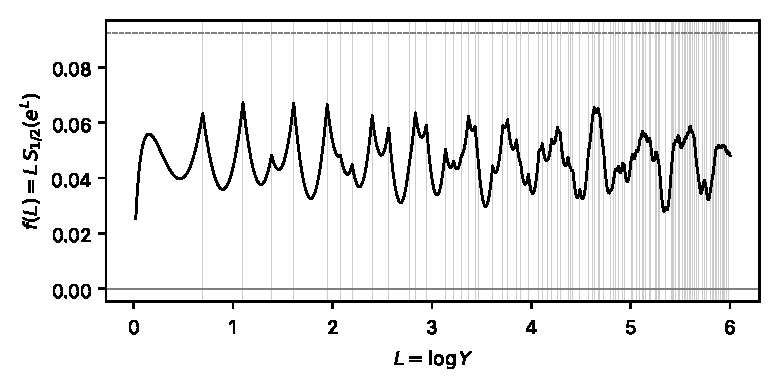
\includegraphics[width=\textwidth]{fig/v3/bo_oscillator.pdf}
\caption{The slack $f(L)$ computed from the primes. Vertical lines are at the logarithms of the prime powers, where $f$ has a downward kink of size $\Lambda(n)/\sqrt n$; between them $f$ is convex. The dashed line is the bound $M=0.092420$.}
\label{bo:fig:osc}
\end{figure}

\paragraph{The picture.} Think of $f$ as the position of a particle and $L$ as time. The pole of $\zeta$ accelerates the particle upward, with a force $e^{L/2}$ that grows exponentially. Each prime power $n$ delivers a downward kick of size $\Lambda(n)/\sqrt n$ at the time $\log n$. The trivial zeros contribute a small force that dies out. Between kicks the motion is convex, since $e^{L/2}>\sum_ke^{-(2k+\frac12)L}$ for $L>0.3$, so the particle can only reach a new maximum at a kick time. RH is the statement that under this exponentially growing push and this discrete train of kicks the particle stays for ever in the band $[0,M]$. Both the push and the accumulated kicks are of size $e^{L/2}$, so the balance must hold to a relative accuracy $e^{-L/2}$ at every time. A zero at distance $d$ off the line is an unstable mode: it adds to $f$ a term of size $e^{dL}/\gamma^2$ that oscillates in sign, and so leaves the band in both directions. This is what has to cancel in the Thorin measure, in its simplest form: an exponential against a sum of point masses on the logarithms of the prime powers, twice integrated, for all time.

\paragraph{The string.} Under RH the same function is $\int(1-\cos(L/\sqrt x))\,\nu(\dd x)$. In the language of Chapter~\ref{b:ch:chain} and of Krein's theory, $\nu$ is the spectral measure of a string whose frequencies are the ordinates $\gamma$, and $\int\cos(L/\sqrt x)\,\nu(\dd x)$ is its wave propagator at time $L$, seen from the end of the string. The bound $0\le f\le2\nu(\mathbb R)$ is then the statement that a wave on a real string is bounded by its initial value, which is true because the frequencies are real. The kinks say that the echoes of the string arrive at the times $\log n$, with amplitudes $\Lambda(n)/\sqrt n$: the primes are the echo times. We offer this as a reading and not as a construction, since the string exists only if RH holds.

\paragraph{Two transforms of one measure.} The chapters on the chain and this chapter study the same measure $\nu$ through two different transforms. Its moments $\int x^n\nu(\dd x)=2\sum_{\gamma>0}\gamma^{-2(n+1)}$ are twice the power sums of the chain, computable from the Taylor coefficients of $\xi$, and they give the rates of the chain: this is route B. Its cosine transform in the variable $\gamma=1/\sqrt x$ is computable from the primes, and it gives the Fej\'er slack: this is route A. Positivity of $\nu$ appears on the first side as the positivity of every rate, and on the second as the single inequality $f\ge0$.

\begin{remark}[How rarely the slack comes near zero]\label{bo:comp:records}
By Proposition~\ref{bo:prop:margin}, $\liminf f=0$ under RH. A scan of $f$ from the zeros with step $0.02$ for $1\le L\le2\times10^5$, using $300$ zeros for the scan and all $6703$ at the candidates, finds its smallest grid value to be $0.01795$, at $L=122021.5$, that is $Y\approx10^{52994}$ (an independent recomputation with $1500$ zeros gives $0.01796$ at $L=122021.525$, and other candidates $0.01809$ at $L=56324.4$ and $0.0184$ to $0.0186$). The minimum for $L\le60$ is $0.02134$ (Remark~\ref{bo:comp:fejer}). The candidate selection used $300$ zeros, with error up to $\pm3\times10^{-3}$, and keeps one minimum per $8000$ in $L$, so $0.01795$ is a grid value and not a proved global minimum; dips are about $0.01$ wide in $L$ and can fall between grid points. Over a range of cutoffs up to $Y=10^{86859}$ no grid value fell below $0.0179$, which is $39$ per cent of the mean $0.0462$.
\end{remark}

The slack does return to zero in the limit, but so slowly that it is invisible: bringing $f$ below $\varepsilon$ requires $\gamma L$ to be close to a multiple of $2\pi$ simultaneously for all zeros with $\gamma^2$ below about $1/\varepsilon$ and for the bulk of those beyond, and on the evidence of the scan the waiting time for such an alignment grows very rapidly as $\varepsilon$ decreases. We have no proof of a rate.

\begin{corollary}[An elementary form]\label{bo:cor:elementary}
Let $A=\frac{\zeta'}{\zeta}(\frac12)=2.68609171$ and $D(Y)=\sum_{k\ge1}\bigl(1-Y^{-(2k+\frac12)}\bigr)/(2k+\frac12)^2$, which increases to $\frac14\psi'(\frac54)=0.29933$. RH holds if and only if, for all $Y>1$,
\[
0\ \le\ 4\sqrt Y-4-A\log Y+D(Y)-\sum_{n\le Y}\frac{\Lambda(n)}{\sqrt n}\,\log\frac Yn\ \le\ M=0.0924199724617,
\]
where $M=4\sum_{\gamma>0}\gamma^{-2}$ (the upper bound may be replaced by any larger constant). Either inequality alone, for all large $Y$, already implies RH.
\end{corollary}

\begin{proof}
The middle expression is $f(\log Y)$, by the first line of the proof of Theorem~\ref{bo:thm:osc}, with $G(\frac12)=2-A$: since $\frac{\xi'}{\xi}(\frac12)=0$ by the functional equation, $G(\frac12)=F(\frac12)=2-\frac{\zeta'}{\zeta}(\frac12)=-0.68609$, which agrees with the digamma value.
\end{proof}

So RH is the statement that one Riesz mean of the von Mangoldt function, $\sum_{n\le Y}\Lambda(n)n^{-1/2}\log(Y/n)$, is equal to an elementary function of $Y$ up to an error that stays in a fixed band of width $0.092420$. The band is absolute: it does not grow with $Y$. Under linear independence of the ordinates $f$ comes arbitrarily close to $M$, so the constant cannot be lowered.

\subsection{The oscillator at every frequency, and the density at level $\alpha$}\label{bo:sec:freq}

The slack at height $t$ is $f_t(L)=L\,S_L(\frac12,t)=L\sum_\rho\Re\kappa_L(\frac12+it-\rho)$, an explicit expression in the primes up to $e^L$; $f_0=f$. The two $2\sin^2$ transforms are dual: $J_\alpha$ is the $2\sin^2$ transform in the frequency $t$ of the prime measure $e^{-\alpha w}\dd R(e^w)$, and $f_t$ is, under RH, the $2\sin^2$ transform in the frequency $L$ of the zero measure, centred at $t$.

\begin{theorem}[Laplace transform of the oscillator]\label{bo:thm:freq}
(a) For real $\lambda>\max(0,\Theta-\frac12)$, $\int_0^\infty e^{-\lambda L}f_t(L)\dd L=\lambda^{-2}\Re\frac{\xi'}{\xi}(\frac12+\lambda+it)$. Hence for $\alpha=\frac12+\delta>\Theta$ (every $\alpha>\frac12$ under RH)
\[
\pi\,u_\alpha(t)=\delta^2\int_0^\infty e^{-\delta L}f_t(L)\dd L,\qquad J_\alpha(t)=\delta^2\int_0^\infty e^{-\delta L}\bigl(f_t(L)-f_0(L)\bigr)\dd L-B_\alpha(t).
\]
(b) Under RH, $f_t(L)=\sum_\rho\frac{2\sin^2((t-\gamma)L/2)}{(t-\gamma)^2}\ge0$ (a term $L^2/2$ if $t=\gamma$), and for $t$ not an ordinate $0\le f_t\le M(t)=2\sum_\rho(t-\gamma)^{-2}$, with $M(0)=M$. The Ces\`aro mean of $f_t$ is $M(t)/2$, so $\pi u_{1/2+\delta}(t)=\frac\delta2M(t)+o(\delta)$.
(c) For $t$ not the ordinate of a zero with $\beta>\frac12$: RH holds if and only if $f_t(L)\ge0$ for all large $L$, if and only if $f_t(L)=O(e^{\varepsilon L})$ for every $\varepsilon>0$; if $t$ is not an ordinate at all, also if and only if $f_t$ is bounded.
\end{theorem}

\begin{proof}
(a) is the Laplace identity in the proof of Theorem~\ref{bo:thm:fejer} at $\alpha=\frac12$ and $s=\frac12+it$; the second formula subtracts the case $t=0$ and uses the ledger. (b) $\Re\kappa_L(ix)=(1-\cos xL)/(Lx^2)$ and $(1-\cos xL)/x^2=\pi L\,\Phi_L(x)$; the Ces\`aro mean of $1-\cos xL$ is $1$ for $x\ne0$, and Abel means agree with Ces\`aro means for bounded functions. (c) is Theorem~\ref{bo:thm:fejer} at $\alpha=\frac12$.
\end{proof}

So the Thorin density at level $\alpha$ is the Abel mean, at rate $\delta=\alpha-\frac12$, of the oscillator at frequency $t$, and the ledger deficit $J_\alpha(t)+B_\alpha(t)$ is the Abel mean of $f_t-f_0$. The oscillator $f_t$ is not uniformly bounded in $t$: under RH $M(t)\ge2\,\mathrm{dist}(t,\{\gamma\})^{-2}$, and for fixed $L$ the $t$ average of $f_t(L)$ is $\frac L2\log\frac t{2\pi}+O(L)$; since $\delta^2\int_0^\infty e^{-\delta L}L\dd L=1$, this is the oscillator image of $\frac12\log\frac t{2\pi}$, the average of $\pi u_\alpha$. The height $t=0$ is special only because $|\gamma|\ge14.13$.

\subsection{Three oscillators: zeta, the control, and random primes}

The oscillator can be run with other kicks. Two comparisons show what is special about the primes.

\paragraph{The control.} The Davenport and Heilbronn function $f_{\rm DH}(s)=\sum a(n)n^{-s}$ has coefficients $a(n)=1,\kappa,-\kappa,-1,0$ for $n\equiv1,2,3,4,0$ modulo $5$ (Section~\ref{ht:sec:dh}). Its logarithmic derivative has coefficients $\Lambda_c=(a\log)*a^{-1}$, where $a^{-1}$ is the Dirichlet inverse of $a$. They are real, of both signs, and supported on all integers prime to $5$, not on prime powers. The completed function has no pole, so there is no exponential push, and its oscillator is
\[
f_c''(L)=-\sum_{k\ge0}e^{-(2k+\frac32)L}-\sum_{n\ge2}\frac{\Lambda_c(n)}{\sqrt n}\,\delta(L-\log n),
\]
with $f_c(L)=L\,c'+\sum_{k\ge0}(1-e^{-(2k+\frac32)L})/(2k+\frac32)^2-\sum_{n\le e^L}\Lambda_c(n)n^{-1/2}(L-\log n)$ and $c'=\frac12\log\frac5\pi+\frac12\psi(\frac34)$. By the proof of Theorem~\ref{bo:thm:osc}, $f_c$ is the sum of $2(\cosh((\rho-\frac12)L)-1)/(\rho-\frac12)^2$ over the pairs of zeros of the control.

\begin{remark}[Computation]\label{bo:comp:controlosc}
We computed $a^{-1}(n)$ and $\Lambda_c(n)$ for all $n\le5\times10^8$ by direct Dirichlet convolution, and from them $f_c(L)$ at $400$ equally spaced values of $L\le20.03$. No zero of the control enters this computation. Up to $L=16$ the result agrees to within $0.02$ with the sum over the control's $304$ zeros on the line below height $420$ and its two lowest quadruples; the difference is the contribution of the zeros not in that list. For $0.5<L<19.5$ it stays between $0.033$ and $0.381$ (an independent zero side run gives $0.0317$ to $0.3700$ without tail). It is first negative at the checkpoint $L=19.58$; the zero side predicted the first sign change at $L=19.57$ (independently $19.575$), from the quadruple at $0.8085\pm85.6993i$, and this is the value of Volume II, Section~\ref{yo:sec:tent}. At $L=19.73$ the prime side value is $-0.035$, while the zero side, truncated at height $420$ plus the two quadruples, gives $-0.0045$ ($+0.0006$ with the mean of the tail): the two differ and the difference is not resolved. % UNVERIFIED: the prime side values of the control were not reproduced (needs the Dirichlet inverse to 5e8)
\end{remark}

So the control fails the criterion from its own coefficients, at the cutoff $Y=3\times10^8$ predicted from its first zeros off the line. This is the same cross check as in the chain chapter, where the negative rates were found from the kernel without knowledge of the zeros; here the instrument is a sum over integers.

\paragraph{Random primes.} In Cram\'er's model each integer $n\ge3$ is declared prime independently with probability $1/\log n$. Give the oscillator a kick $\log n/\sqrt n$ at time $\log n$ for each such $n$. The mean kick rate matches the push, and the fluctuation of $f$ about its mean is $-\sum(\xi_n-1/\log n)\log n\,n^{-1/2}(L-\log n)$, a sum of independent terms with variance
\[
\int_0^L(w-1)(L-w)^2\dd w=\frac{L^4}{12}-\frac{L^3}{3}
\]
(exact; it vanishes at $L=4$, where the observed value is not zero, because the model treats $n$ below $e^4$ crudely).
\begin{remark}[Computation]\label{bo:comp:random}
Over $40$ realisations with $n\le10^7$, the standard deviation of $f$ is $2.6$, $15.2$, $38.2$ and $72.2$ at $L=4,8,12$ and $16.1$. The last is $780$ times the width $0.092420$ of the band in which the true $f$ lies (Figure~\ref{bo:fig:three}). The observed standard deviations run $11$ to $16$ per cent above the exact ones at $L=8$ to $16$. % UNVERIFIED: not rerun
\end{remark}

\begin{figure}[ht]
\centering
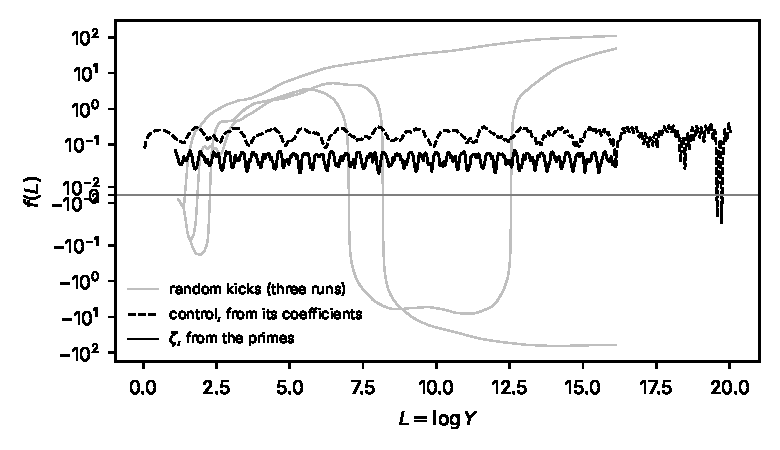
\includegraphics[width=\textwidth]{fig/v3/bo_three.pdf}
\caption{Three oscillators on a scale that is linear near zero and logarithmic beyond $0.05$: the slack $f$ for $\zeta$ from the primes, the control from its Dirichlet coefficients, and three runs with random kicks.}
\label{bo:fig:three}
\end{figure}

\paragraph{What the comparison shows.} With random kicks the particle wanders like $L^2$: there is no exponential instability, which corresponds to the fact that Cram\'er's model has square root cancellation, but there is no band either. With the control's kicks the particle stays in a band for a long time, because most of its zeros are on the line, and then leaves exponentially when the first unstable mode has grown large enough. With the true primes it stays in a band of width $0.092420$ for as far as can be computed, and for ever if RH holds. So boundedness of $f$ asks for more than square root cancellation in $\Psi(y)-y$. It asks that the kicks be the echoes of a string: that the measure $\sum\Lambda(n)n^{-1/2}\delta_{\log n}-e^{L/2}\dd L$ be, up to the archimedean term, the second derivative of a function of the form $\int(1-\cos(L/\sqrt x))\nu(\dd x)$ with $\nu$ positive and finite. Cram\'er's primes satisfy the estimate that RH implies for $\Psi$ and fail this; the control satisfies a functional equation and fails this. In the language of Section~\ref{route:sec:filters}, the oscillator separates the two things a proof must use, the functional equation and the Euler product, more cleanly than the other instruments: remove the first and the band is lost to a random walk, remove the second and it is lost to an exponential.

\subsection{The oscillator in detail}\label{bo:sec:oscdetail}

This subsection looks at the oscillator of Theorem~\ref{bo:thm:osc} as a dynamical system: what its equation is, what its velocity is, how its position and velocity are distributed over time, and how large and how long its swings are.

\paragraph{What the equation is.} The sum over zeros in Theorem~\ref{bo:thm:osc} gives $f''(L)=\sum_\rho e^{(\rho-\frac12)L}$ as distributions on $L>0$ (after pairing $\rho$ with $1-\rho$), so the equation of motion says
\[
\sum_{n\ge2}\frac{\Lambda(n)}{\sqrt n}\,\delta(L-\log n)=e^{L/2}-\sum_\rho e^{(\rho-\frac12)L}-\sum_{k\ge1}e^{-(2k+\frac12)L}.
\]
This is the explicit formula of Riemann, von Mangoldt, Guinand and Weil, $\dd\Psi(x)=\bigl(1-\sum_\rho x^{\rho-1}-\sum_kx^{-2k-1}\bigr)\dd x$, written in the variable $L=\log x$ and multiplied by $x^{-1/2}$. The oscillator is therefore the explicit formula integrated twice, and it is not a new identity. Integrating twice does two things. It makes the sum over zeros absolutely convergent after pairing, with terms of size $\gamma^{-2}$ in place of $\gamma^{-1}$, and it gives a function whose sign can be tested, so that Landau's theorem turns the explicit formula into the one sided criterion of Theorem~\ref{bo:thm:fejer}.

\begin{proposition}[Velocity]\label{bo:prop:velocity}
Let $E(Y)=(\Psi(Y)-Y)/\sqrt Y$. Unconditionally, for $L>0$ (right derivative at the kicks),
\[
f'(L)=1-\frac{\zeta'}{\zeta}\Bigl(\frac12\Bigr)-E(e^L)-\frac12\int_0^LE(e^u)\dd u+\sum_{k\ge1}\frac{e^{-(2k+\frac12)L}}{2k+\frac12}.
\]
\end{proposition}

\begin{proof}
Differentiating the formula for $f$ in the proof of Theorem~\ref{bo:thm:osc} gives $f'(L)=G(\frac12)+2(e^{L/2}-1)+\sum_ke^{-a_kL}/a_k-\sum_{n\le e^L}\Lambda(n)n^{-1/2}$. With $Y=e^L$, $\sum_{n\le Y}\Lambda(n)n^{-1/2}-2(\sqrt Y-1)=\int_1^Yy^{-1/2}\dd R(y)=E(Y)+1+\frac12\int_1^YR(y)y^{-3/2}\dd y$, using $R(1)=-1$, and the last integral is $\int_0^LE(e^u)\dd u$. Finally $G(\frac12)-1=1-\frac{\zeta'}{\zeta}(\frac12)$.
\end{proof}

So the velocity of the oscillator is, up to sign, the normalised error in the prime number theorem, plus a running average of the same error. Under RH the mean of $f'$ is zero (Proposition~\ref{bo:prop:averages}) and so is the mean of $E(e^u)$ (it is a sum of $e^{i\gamma u}/\rho$), hence the running integral $\frac12\int_0^LE(e^u)\dd u$ has Bohr mean $1-\frac{\zeta'}{\zeta}(\frac12)=-1.6861$ but no limit: it is this constant plus a bounded almost periodic function, $\sum_\gamma\cos(\gamma L)\cdot O(\gamma^{-2})$, of amplitude about $0.02$, and the improper integral $\int_0^\infty E(e^u)\dd u$ does not converge. The value of the running integral from the primes to $10^9$ at $L=\log10^9$ is $-1.6920$, which differs from the mean by an amount of that size. % UNVERIFIED: running value not rechecked
The identity of the proposition holds on a grid of $60000$ values of $L$ to $8\times10^{-4}$, the error of the trapezoid rule, and $f'$ and $-E$ have correlation $0.971$ for $L\ge4$. The coefficient of the trivial zero sum was checked by finite differences at $L=0.5$ ($0.02835$ both ways).

\begin{proposition}[Time averages]\label{bo:prop:averages}
Assume RH, and let $m_\gamma$ be the multiplicity of the zero $\frac12+i\gamma$. Then $f$ is almost periodic with frequencies the ordinates, $f'$ lies in Besicovitch's space $B^2$, and, the sums running over distinct ordinates,
\begin{gather*}
\langle f\rangle=2\sum_{\gamma>0}\frac{m_\gamma}{\gamma^2},\qquad \operatorname{Var}f=2\sum_{\gamma>0}\frac{m_\gamma^2}{\gamma^4},\\
\langle f'\rangle=0,\qquad \langle f'^2\rangle=2\sum_{\gamma>0}\frac{m_\gamma^2}{\gamma^2}.
\end{gather*}
In particular $\langle f'^2\rangle\ge\langle f\rangle$, with equality if and only if every zero is simple.
\end{proposition}

\begin{proof}
$f=\sum_{\gamma>0}2m_\gamma(1-\cos\gamma L)/\gamma^2$ converges uniformly, so Parseval's identity for almost periodic functions gives the mean and the variance. By Proposition~\ref{bo:prop:velocity}, $f'$ is $-E(e^L)$ plus a bounded almost periodic function and a decaying term, and $E(e^L)$ lies in $B^2$ under RH (Cram\'er~\cite{Cramer}); its Bohr Fourier coefficients are those of the termwise derivative $f'=\sum_{\gamma>0}2m_\gamma\sin(\gamma L)/\gamma$, whose coefficients are square summable, so Parseval gives the mean square. Since $m_\gamma^2\ge m_\gamma$ with equality only for $m_\gamma=1$, the last statement follows.
\end{proof}

The mean square of the velocity is, through Proposition~\ref{bo:prop:velocity}, Cram\'er's mean square of the normalised Chebyshev error, a classical result. What the oscillator adds is the comparison with the mean position: kinetic and potential averages agree exactly when the zeros are simple.

\begin{remark}[Computation]\label{bo:comp:oscdeep}
From the primes to $10^9$, with $f$ and $f'$ on $60000$ values of $L$ and averages over $4\le L\le20.72$:
\begin{center}\small
\begin{tabular}{@{}lcc@{}}
\toprule
& primes to $10^9$ & from the zeros under RH\\
\midrule
$\langle f\rangle$ & $0.04623$ & $0.04621$\\
$\operatorname{Var}f$ & $0.000074$ & $0.000074$\\
$\langle f'\rangle$ & $+0.002$ & $0$\\
$\langle f'^2\rangle$ & $0.046$ & $0.04621$\\
\bottomrule
\end{tabular}
\end{center}
The position stays in $[0.0215,0.0689]$ (an independent recomputation gives $[0.02152,0.06890]$). The velocity stays within about $\pm0.75$; its extremes depend on the grid, since $f'$ jumps at the prime powers (two recomputations give a minimum of $-0.77$ and $-0.71$), and the last digits are not settled. Over every prime power $100<n\le10^9$ the error $E$ lies in $[-0.751,0.791]$, with the extremes at $n\approx3.69\times10^7$ and $1.10\times10^8$. % UNVERIFIED: E extremes not rerun
\end{remark}

The equality $\langle f'^2\rangle=\langle f\rangle$ holds to two digits, which is what simple zeros require. Simplicity of the zeros is known numerically far beyond this range, so this is a check of the equation, not new evidence.

\begin{figure}[ht]
\centering
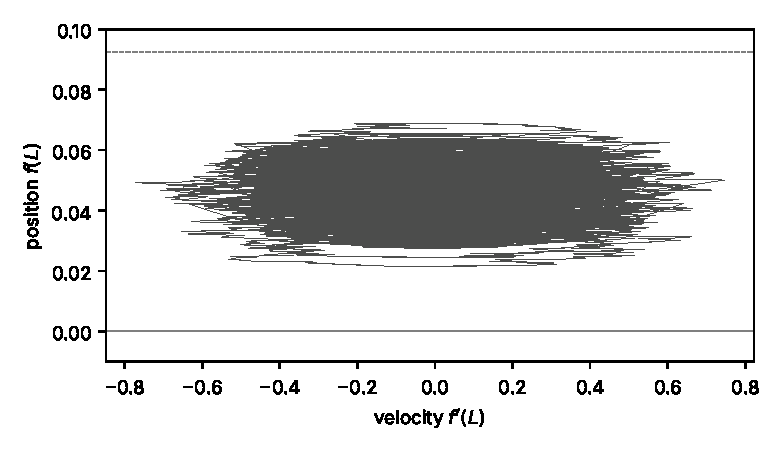
\includegraphics[width=\textwidth]{fig/v3/bo_phase.pdf}
\caption{Phase portrait of the oscillator from the primes to $10^9$, for $4\le L\le20.72$: position $f$ against velocity $f'$. The position stays between the lines $0$ and $M=0.092420$.}
\label{bo:fig:phase}
\end{figure}
% The velocity range printed on the original axes is about -0.77 to 0.75; one recomputation gave -0.71. The figure may need redrawing on a finer grid.

\paragraph{Unbounded speed in a bounded band.} By Littlewood's theorem~\cite{Littlewood14} $\Psi(x)-x$ is larger than $c\sqrt x\log\log\log x$ in absolute value, with both signs, for arbitrarily large $x$. By Proposition~\ref{bo:prop:velocity} the velocity $f'$ is then unbounded above and below, while under RH the position stays in a band of width $M$. Figure~\ref{bo:fig:phase} shows the shape this forces on the trajectory: wide in velocity and thin in position. It also gives a quantitative constraint on the error term.

\begin{corollary}[Short swings]\label{bo:cor:swings}
Assume RH. If $f'\ge v>0$ almost everywhere on an interval $[L_1,L_2]$, or $f'\le-v$ there, then $v\,(L_2-L_1)\le M$. Equivalently, up to the running average in Proposition~\ref{bo:prop:velocity}, a value $|E(x)|\ge v$ of one sign can persist only over a range of $x$ of ratio at most $e^{M/v}$.
\end{corollary}

\begin{proof}
$|f(L_2)-f(L_1)|=\bigl|\int_{L_1}^{L_2}f'\bigr|\ge v(L_2-L_1)$, and both values lie in $[0,M]$.
\end{proof}

In the data the swings are much shorter than the corollary allows. The longest run with $f'\ge0.1$ has length $0.127$ in $L$, and the longest with $|f'|\ge0.4$ has length $0.018$. The products $v(L_2-L_1)$ never exceed $0.020$, a fifth of the bound. % UNVERIFIED: swing lengths from the draft, not rerun
The Chebyshev error is not a slowly varying function of $x$. It is a superposition of the waves $\sin(\gamma\log x)/\gamma$, and since no single low frequency dominates, it changes sign before it can carry the oscillator far. The transfer from $f'$ to $E$ ignores the remaining terms of Proposition~\ref{bo:prop:velocity}, which are bounded but not negligible.

\paragraph{What this means for a proof.} A proof that the oscillator stays in its band must control the position, an integral of the velocity, while the velocity itself is unbounded. Bounds on $|\Psi(x)-x|$, of the kind that zero density or large sieve methods give, act on the velocity and lose a factor of the length of the time interval when integrated. What is needed is a bound on the cancellation of the velocity over time, that is on $\int_{L_1}^{L_2}E(e^u)\dd u$ uniformly in $L_1$ and $L_2$. That is a statement about the averages of the Chebyshev error over multiplicative intervals of every length.

\subsection{The distribution of the oscillator}\label{bo:sec:oscdist}

The band $[0,M]$ is where the oscillator must stay under RH. This subsection asks how much of the band it actually uses, in the sense of time spent, and gives a quantitative form of the observation that the walls are approached only very rarely.

\begin{proposition}[Limiting distribution]\label{bo:prop:oscdist}
Assume RH. Then $f$ and $f'$ have limiting distributions in $L$: for continuous bounded $g$, $\frac1X\int_0^Xg(f(L))\dd L$ converges, and likewise for $f'$. If moreover the positive ordinates are linearly independent over $\mathbb Q$ (the hypothesis LI, which implies that the zeros are simple), the limits are the laws of
\[
\mathcal F=\sum_{\gamma>0}\frac{2}{\gamma^2}(1-\cos\theta_\gamma),\qquad \mathcal V=\sum_{\gamma>0}\frac{2}{\gamma}\sin\theta_\gamma,
\]
with $\theta_\gamma$ independent and uniform on $[0,2\pi)$. The characteristic function of $\mathcal F$ is $\prod_{\gamma>0}e^{2i\tau/\gamma^2}J_0(2\tau/\gamma^2)$.
\end{proposition}

\begin{proof}
By Theorem~\ref{bo:thm:osc}, $f$ is a uniformly convergent sum of $2(1-\cos\gamma L)/\gamma^2$, so it is uniformly almost periodic and has a limiting distribution by the Kronecker and Weyl theorem applied to finite truncations, with the remainder uniformly small. For $f'$ the series converges in the Besicovitch mean square (Proposition~\ref{bo:prop:averages}), which is enough for the same conclusion; this is the argument of Rubinstein and Sarnak~\cite{RubinsteinSarnak94} for the normalised prime counting error. Under LI the flow $L\mapsto(\gamma L)_\gamma$ is equidistributed on the torus, which gives independent uniform phases.
\end{proof}

The law of $\mathcal F$ is supported on all of $[0,M]$, since $\sum_\gamma4/\gamma^2=M$, but its mass sits in the middle. Two consequences can be made exact.

\begin{corollary}[Wall probabilities]\label{bo:cor:walls}
Under LI, for every $s>0$ and $c>0$,
\begin{gather*}
\mathbb P(\mathcal F<c)\le e^{sc}\prod_{\gamma>0}e^{-2s/\gamma^2}I_0\bigl(2s/\gamma^2\bigr),\\
\mathbb P(\mathcal F>c)\le e^{-sc}\prod_{\gamma>0}e^{2s/\gamma^2}I_0\bigl(2s/\gamma^2\bigr).
\end{gather*}
\end{corollary}

\begin{proof}
Markov's inequality applied to $e^{-s\mathcal F}$ and $e^{s\mathcal F}$, with $\E e^{\pm sa(1-\cos\theta)}=e^{\pm sa}I_0(sa)$.
\end{proof}

Both bounds can be evaluated rigorously with any finite list of zeros. Dropping zeros keeps the lower tail bound valid but weakens it, since every dropped factor $e^{-2s/\gamma^2}I_0(2s/\gamma^2)$ is at most $1$. For the upper tail the zeros above the list add at most $\sum_{\gamma>T}4/\gamma^2$ to $\mathcal F$, which is $7.3\times10^{-4}$ for $T=7000$, and this is subtracted from $c$.

\begin{remark}[Computation]\label{bo:comp:oscli}
With the $6703$ zeros below $7000$, the law of $\mathcal F$ by Fourier inversion of the product of Bessel functions, and the law of $\mathcal V$ likewise, compared with the primes to $10^9$ over $4\le L\le20.72$:
\begin{center}\small
\begin{tabular}{@{}lccccc@{}}
\toprule
quantile & $1\%$ & $10\%$ & $50\%$ & $90\%$ & $99\%$\\
\midrule
$f$, under LI & $0.02837$ & $0.03477$ & $0.04621$ & $0.05765$ & $0.06404$\\
$f$, primes & $0.02855$ & $0.03491$ & $0.04617$ & $0.05772$ & $0.06317$\\
$f'$, under LI & $-0.494$ & $-0.277$ & $0.000$ & $0.277$ & $0.494$\\
$f'$, primes & $-0.481$ & $-0.280$ & $0.000$ & $0.282$ & $0.486$\\
\bottomrule
\end{tabular}
\end{center}
The standard deviation of $f$ is $0.00862$ under LI (independently $\sqrt{2\sum\gamma^{-4}}=0.0086227$) and $0.00861$ from the primes. The bounds of Corollary~\ref{bo:cor:walls}, optimised over $s$, give
\begin{center}\small
\begin{tabular}{@{}lccccc@{}}
\toprule
$c$ & $0.001$ & $0.005$ & $0.01$ & $0.015$ & $0.02$\\
$\log_{10}\mathbb P(\mathcal F<c)\le$ & $-770$ & $-84$ & $-23$ & $-9.4$ & $-4.3$\\
\midrule
$c$ & $0.07$ & $0.075$ & $0.08$ & $0.085$ & $0.09$\\
$\log_{10}\mathbb P(\mathcal F>c)\le$ & $-3.0$ & $-6.3$ & $-15$ & $-42$ & $-255$\\
\bottomrule
\end{tabular}
\end{center}
% UNVERIFIED: the quantile and Chernoff tables were not reproduced (only the standard deviation was)
\end{remark}

\begin{figure}[ht]
\centering
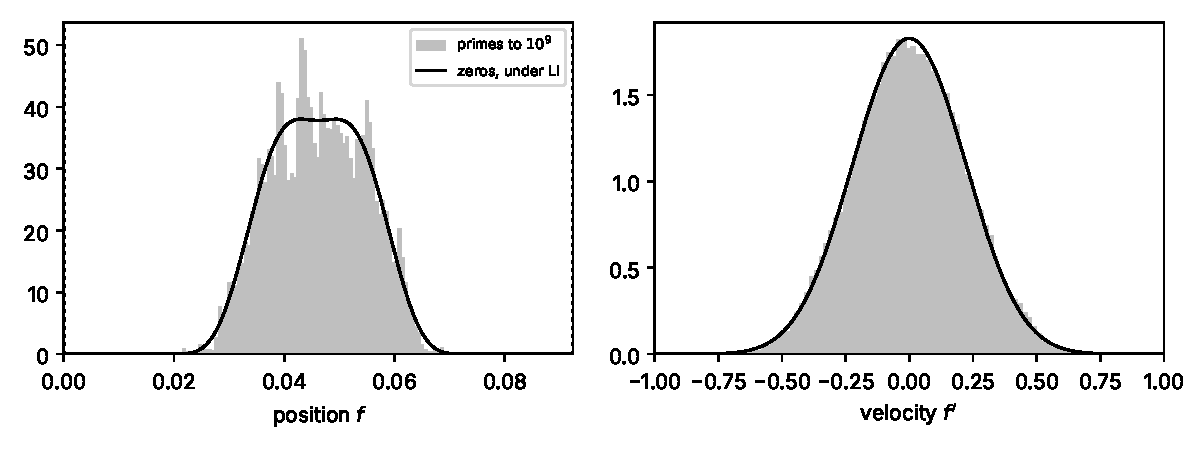
\includegraphics[width=\textwidth]{fig/v3/bo_li.pdf}
\caption{Time spent by the oscillator, from the primes to $10^9$ (histograms), against the laws of $\mathcal F$ and $\mathcal V$ computed from the zeros under LI (curves). Left: position, with the band $[0,M]$ dotted. Right: velocity.}
\label{bo:fig:li}
\end{figure}

\paragraph{What this says about the band.} Under RH and LI the oscillator spends a proportion of logarithmic time below $0.01$ that is less than $10^{-23}$, and below $0.005$ less than $10^{-84}$. The position $f$ comes near $0$ only when $\gamma L$ is close to a multiple of $2\pi$ for every low lying ordinate at once, a simultaneous return of the zero torus to its origin, and Kronecker's theorem says such returns happen, which is why $\liminf f=0$ (Proposition~\ref{bo:prop:margin}), but the computation shows how rarely.

The law also predicts the scan of Remark~\ref{bo:comp:records}, which found a smallest grid value $0.01795$ for $L\le2\times10^5$. Under LI, $\mathbb P(\mathcal F<0.018)=8\times10^{-8}$, so a range of length $2\times10^5$ spends a total time of about $0.016$ below $0.018$; a dip near the minimum lasts about $0.01$ in $L$, so one or two dips to that level are expected, which is what the scan found.

First, no computation of primes will ever see the oscillator near its lower wall: the minimum $0.0215$ observed up to $10^9$ is far above the minimum of the law. A failure of RH would appear in the oscillator first as a slowly growing oscillation $e^{(\beta-\frac12)L}\cos(\gamma L)/\gamma^2$ with $\beta-\frac12$ small, and not as a crossing of the wall at any accessible height.

Second, the agreement in the tables is a check on the zeros and the primes together, not evidence for RH: the first $6703$ zeros are known to be on the line, and the law of $\mathcal F$ depends on the low zeros almost entirely, since $\sum_{\gamma>7000}2/\gamma^2$ is $3.7\times10^{-4}$, under $1\%$ of the mean. What the oscillator offers a proof is the shape of the target. RH is equivalent to a two sided bound on a function whose time distribution has standard deviation $0.0086$ and sits five standard deviations from either wall, and the difficulty is entirely in the exceptional times, which are the near returns of the zeros.

\subsection{The oscillator of an $L$ function}\label{bo:sec:oscopen}

The oscillator is not special to $\zeta$. This subsection builds it for any $L$ function with an Euler product and a functional equation, finds that it measures the order of the central zero with an error that falls like $1/h^2$ in the logarithm of the cutoff, tests this on four elliptic curves, and lists what remains open.

\paragraph{The oscillator of an $L$ function.} Let $L(s)=\sum a_nn^{-s}$ be normalised so that the centre is $s=\frac12$, with completed function $\Lambda(s)$ entire, of order one, $\Lambda(s)=\pm\Lambda(1-s)$ and no pole. Write $-\frac{L'}{L}(s)=\sum c(n)n^{-s}$, and let the trivial zeros be the points $t$ where the gamma factor has poles. Put, pairing $\rho$ with $1-\rho$ (the unpaired series does not converge absolutely, its terms having size $L/|\gamma|$),
\[
f(L)=\sum_{\{\rho,1-\rho\}}\Bigl[\frac{e^{(\rho-\frac12)L}-1-(\rho-\frac12)L}{(\rho-\frac12)^2}+\frac{e^{-(\rho-\frac12)L}-1+(\rho-\frac12)L}{(\rho-\frac12)^2}\Bigr],
\]
over pairs of nontrivial zeros with multiplicity. For $\zeta$ this is the oscillator of Theorem~\ref{bo:thm:osc} with the pole removed.

\begin{theorem}[Oscillator of an $L$ function]\label{bo:thm:oscL}
On $L>0$, as distributions, $f''(L)=\sum_\rho e^{(\rho-\frac12)L}=-\sum_n c(n)n^{-1/2}\delta(L-\log n)-\sum_te^{(t-\frac12)L}$. Hence $f=a+bL-P-Q$ with constants $a$, $b$, where $P(L)=\sum_{\log n\le L}c(n)n^{-1/2}(L-\log n)$ and $Q''=\sum_te^{(t-\frac12)L}$. If all nontrivial zeros are on the line, and $m_0$ is the order of the zero at $s=\frac12$,
\[
f(L)=\frac{m_0}{2}L^2+\Phi(L),\qquad 0\le\Phi(L)\le W=2\sum_{\gamma\ne0}\frac{m_\gamma}{\gamma^2}.
\]
\end{theorem}

\begin{proof}
The first identity is the explicit formula, as in Theorem~\ref{bo:thm:osc}. A zero at the centre gives the limit $L^2/2$ of the summand. A pair $\frac12\pm i\gamma$ gives $2(1-\cos\gamma L)/\gamma^2$, the linear terms cancelling, and this lies in $[0,4/\gamma^2]$.
\end{proof}

So a central zero is invisible to the band criterion for $\zeta$ only because $\zeta(\frac12)\ne0$. For an $L$ function that vanishes at the centre the oscillator grows like a parabola, and its curvature is the order of vanishing. The unknown constants $a$, $b$ are removed by a second difference.

\begin{corollary}[Central order from the primes]\label{bo:cor:rank}
Let $h>0$ and $\hat r(h)=-\bigl(\Delta_h^2P+\Delta_h^2Q\bigr)/h^2$, where $\Delta_h^2g=g(0)-2g(h)+g(2h)$. Under GRH, $\hat r(h)-m_0=\Delta_h^2\Phi/h^2$, so $|\hat r(h)-m_0|\le2W/h^2$. The quantity $\hat r(h)$ uses only $c(n)$ for $n\le e^{2h}$.
\end{corollary}

\begin{proof}
$\Delta_h^2(a+bL)=0$ and $\Delta_h^2\frac{m_0}{2}L^2=m_0h^2$, so $\hat r(h)-m_0=\Delta_h^2\Phi/h^2$, and $|\Delta_h^2\Phi|\le2W$ since $\Phi\in[0,W]$.
\end{proof}

The constant $W$ can itself be bounded from the primes, given $m_0$. At $s=\frac32$ the Euler product converges absolutely, and pairing $\rho$ with $1-\bar\rho$ gives $\frac{\Lambda'}{\Lambda}(\frac32)=\sum_\rho\Re\frac1{\frac32-\rho}$, every term positive. A central zero contributes $1$, so unconditionally $m_0\le\frac{\Lambda'}{\Lambda}(\frac32)$ (the analytic order; compare Proposition~\ref{iw:prop:rank}, a bound in the style of Mestre). Under GRH the remaining sum is $S=\sum_{\gamma\ne0}1/(1+\gamma^2)$ with $S=\frac{\Lambda'}{\Lambda}(\frac32)-m_0$; the first ordinate $\gamma_1$ satisfies $2/(1+\gamma_1^2)\le S$, and $1/\gamma^2\le(1+\gamma_1^{-2})/(1+\gamma^2)$, so
\[
W\le2\bigl(1+\gamma_1^{-2}\bigr)S,\qquad \gamma_1^2\ge\frac2S-1 .
\]

\begin{remark}[Computation]\label{bo:comp:rank}
For the elliptic curves $11a$, $37a$, $389a$ and $5077a$, of ranks $0$ to $3$, with $a_p$ for $p\le10^6$ by point counting and $L(s)=L(E,s+\frac12)$, so that the trivial zeros are $-\frac12-k$ and $Q(L)=\operatorname{Li}_2(e^{-L})$:
\begin{center}\small
\begin{tabular}{@{}lccccc@{}}
\toprule
curve & rank & $\frac{\Lambda'}{\Lambda}(\frac32)$ & $W\le$ & $\hat r$ at $X=10^6$ & $2W/h^2$\\
\midrule
$11a$ & $0$ & $0.253$ & $0.58$ & $-0.007$ & $0.024$\\
$37a$ & $1$ & $1.374$ & $0.92$ & $0.988$ & $0.039$\\
$389a$ & $2$ & $2.778$ & $2.55$ & $1.990$ & $0.107$\\
$5077a$ & $3$ & $4.331$ & $7.95$ & $2.971$ & $0.333$\\
\bottomrule
\end{tabular}
\end{center}
Here $h=\frac12\log10^6=6.91$, and $\frac{\Lambda'}{\Lambda}(\frac32)$ is computed from $n\le10^6$ with error below $0.004$. The column $W\le$ uses the known rank as $m_0$. Every $\hat r$ is within $0.03$ of the rank. The classical sum $\frac12-\frac1{\log X}\sum_{p\le X}a_p\log p/p$ is off by $0.14$ to $0.23$ at the same $X$ (Figure~\ref{bo:fig:rank}); it is known to tend to the rank under GRH only together with a further hypothesis on the prime sum (Kuo and Murty~\cite{KuoMurty05}), which we have not checked. % UNCHECKED: references for the classical estimator not read; TODO for the authors: Goldfeld's 1982 estimator has no bibliography entry and its name was cut
Unconditionally, the bound $m_0\le\frac{\Lambda'}{\Lambda}(\frac32)$ gives $L(11a,1)\ne0$, analytic rank at most $1$ for $37a$, and at most $2$ and $4$ for the others.
\end{remark}

The table is a consistency check and not a determination of the ranks, because $W$ was computed from the rank it is meant to certify. A test that does not use the rank accepts each candidate $m_0$ with $|\hat r-m_0|\le2W(m_0)/h^2$. It excludes the wrong candidates for $11a$ (by the unconditional bound) and for $37a$, but for $389a$ the candidate $m_0=1$ gives $\frac{\Lambda'}{\Lambda}(\frac32)-m_0=1.778$, $W\le32$ and $2W/h^2=1.34>|1.990-1|$, so it is not excluded, and for $m_0=0$ and for $5077a$ at $m_0\le2$ the bound on $W$ is vacuous. % UNVERIFIED: W4 did not recompute the elliptic curve table; the non circular reading follows referee U09 M11

\begin{figure}[ht]
\centering
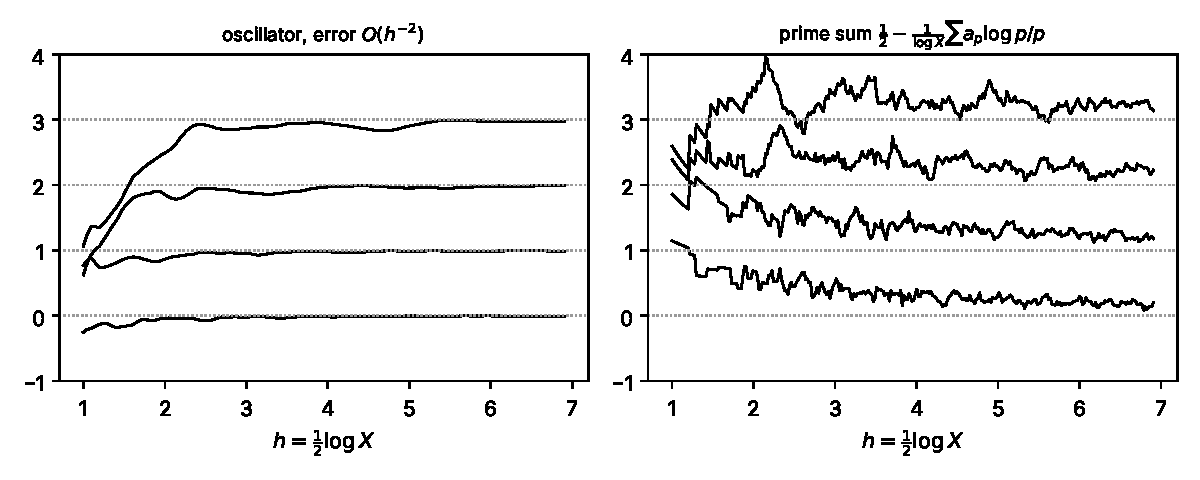
\includegraphics[width=\textwidth]{fig/v3/osc_rank.pdf}
\caption{Order of the central zero for four elliptic curves of ranks $0,1,2,3$, against $h=\frac12\log X$. Left: the oscillator estimate $\hat r(h)$ of Corollary~\ref{bo:cor:rank}. Right: the classical prime sum. Dotted lines are the ranks.}
\label{bo:fig:rank}
\end{figure}

\section{The value distribution of $J_\alpha$}\label{bo:sec:values}

For $\frac12<\alpha<1$ and $t$ uniform on $[0,T]$, what do the blocks of the ledger do? Since $J_\alpha(t)=F(\alpha)+\Re\frac{\zeta'}{\zeta}(\alpha+it)+\frac{\alpha-1}{(\alpha-1)^2+t^2}$ (the last term is the pole at $s=1$), the value distribution of $J_\alpha$ is that of $\Re\frac{\zeta'}{\zeta}(\alpha+it)$ shifted by $F(\alpha)=-\frac{\zeta'}{\zeta}(\alpha)-\frac1{\alpha-1}$. Here $J_\alpha$ means $J^{\rm cont}_\alpha$ of Remark~\ref{bo:rem:scope}, which is the integral of Theorem~\ref{bo:thm:ledger} when $\alpha>\Theta$. Let $(X_p)$ be independent and uniform on the unit circle, $X(n)=\prod_pX_p^{v_p(n)}$, and $Z_\alpha=-\sum_n\Lambda(n)n^{-\alpha}X(n)=-\sum_p\frac{(\log p)p^{-\alpha}X_p}{1-p^{-\alpha}X_p}$. The first series converges in $L^2$ and the second almost surely, and they agree.

\begin{theorem}[Limiting law]\label{bo:thm:limitlaw}
For fixed $\alpha\in(\frac12,1)$ and every bounded continuous $\varphi$, $\frac1T\int_0^T\varphi\bigl(\frac{\zeta'}{\zeta}(\alpha+it)\bigr)\dd t\to\E\varphi(Z_\alpha)$ (complex values), with no hypothesis. Hence $J_\alpha(t)\Rightarrow F(\alpha)+\Re Z_\alpha$, and the limit law has a $C^\infty$ density with support $\mathbb R$.
\end{theorem}

This is due to Kershner and Wintner~\cite{KershnerWintner37}; the density theory in the $L'/L$ setting is Ihara's theory of $M$ functions~\cite{Ihara08}. The proof that follows uses only the zero density estimates, which confine the zeros to the right of $\alpha-\varepsilon$ to a set of heights of measure $o(T)$.

\begin{proof}[Outline]
Fix $\frac12<\sigma_0<\alpha$ and let $E_T$ be the set of $t\in[T,2T]$ within $2\log T$ of the ordinate of a zero with $\beta>\sigma_0$; $\operatorname{meas}E_T\ll T^{1-\eta(\sigma_0)}\log^{B}T$ by Ingham's estimate. Off $E_T$, Mellin inversion and the classical bound for $\frac{\zeta'}{\zeta}$ in terms of nearby zeros give, with $y=(\log T)^{4/(\alpha-\sigma_0)}$, $|\frac{\zeta'}{\zeta}(\alpha+it)+\sum_n\Lambda(n)n^{-\alpha-it}e^{-n/y}|\le C/\log T$. The Montgomery and Vaughan mean value theorem~\cite{MV74} shows that this smoothed Dirichlet polynomial differs in mean square from $-\sum_{n\le N}\Lambda(n)n^{-\alpha-it}$ by at most $\varepsilon_N=\sum_{n>N}\Lambda(n)^2n^{-2\alpha}$ plus a term that vanishes as $T\to\infty$. For fixed $N$ the finite sum is a continuous function of $(t\log p/2\pi)_{p\le N}$, equidistributed on the torus by Kronecker and Weyl since the $\log p$ are linearly independent over $\mathbb Q$. Billingsley's Theorem 3.2 closes the argument, and dyadic blocks give $[0,T]$. For the density, $W_p=\Re$ of the summand for $p$ has two nondegenerate critical points in the phase, so its characteristic function is $O(|\xi|^{-1/2})$ (van der Corput), and a product of $N$ such factors decays like $|\xi|^{-N/2}$; the support is $\mathbb R$ because the ranges of the $W_p$ have divergent endpoint series with terms tending to $0$. % TODO for the authors: no bibliography entry for Billingsley, Theorem 3.2
\end{proof}

\begin{proposition}[Mean and variance]\label{bo:prop:meanvar}
(a) The limit law has mean $F(\alpha)$ for $J_\alpha$ and variance $V_\alpha=\frac12\sum_n\Lambda(n)^2n^{-2\alpha}=\frac12\bigl[(\frac{\zeta'}{\zeta})'(2\alpha)-\sum_p\frac{(\log p)^2p^{-4\alpha}}{(1-p^{-2\alpha})^2}\bigr]$, all moments are finite and $V_\alpha=\frac1{8\delta^2}+O(1)$ as $\delta\to0+$. For example $V_{0.55}=49.4468$, $V_{0.6}=12.0906$, $V_{0.75}=1.79571$, $V_{0.9}=0.656060$. (b) Time moments of every order on $[T,2T]$ minus a set of measure $\ll T^{1-\eta}$ converge to the model moments, and the first absolute moment converges on all of $[0,T]$. Moments of order $k\ge2$ on all of $[0,T]$ converge if $\Theta<\alpha$; unconditionally this is open, because a zero within $c/\log T$ of the line $\Re s=\alpha$ would contribute a spike of mean square $\gg1/\eta$ over a window of length $\eta$.
\end{proposition}

\begin{proof}
(a) $\E Z_\alpha^2=0$ since $\E X(n)X(m)=0$ for $nm>1$, so $\operatorname{Var}\Re Z_\alpha=\frac12\E|Z_\alpha|^2=V_\alpha$. The closed form uses $\sum\Lambda(n)\log n\,n^{-s}=(\frac{\zeta'}{\zeta})'(s)$ and $\Lambda(n)\log n-\Lambda(n)^2=(k-1)(\log p)^2$ for $n=p^k$. The behaviour at $\delta\to0$ is the double pole of $(\frac{\zeta'}{\zeta})'$ at $1$. (b) The same argument as in the outline, with Montgomery and Vaughan~\cite{MV74} for even moments of Dirichlet polynomials of length $T^{1/2}$ and uniform integrability.
\end{proof}

\begin{remark}[Computation]\label{bo:comp:values}
With $t$ uniform on $[1000,7000]$ and $40000$ samples of $J_\alpha$ computed from the $8000$ zeros: at $\alpha=\frac34$ the mean is $-0.620$ against $F=-0.6276$ and the variance $1.720$ against $V=1.7957$ ($4.2$ per cent below); at $\alpha=\frac78$ the mean is $-0.598$ against $F=-0.6015$ and the variance $0.746$ against $V=0.7545$ ($1.1$ per cent below). A random phase model with primes to $2\times10^5$ reproduces $V$ ($1.750$ and $0.761$). The excess kurtosis of $J_\alpha$ is $-0.90$ and $-0.53$, against about $0$ in the model: at accessible heights the law is sub Gaussian, shaped by the rigid comb of zeros. The governing parameter is $\delta\log(t/2\pi)/2\pi$, the Poisson width over the mean zero spacing, which is about $0.26$ and $0.41$ here, and the Euler product law describes the data only when it is large. The minimum of $\pi u_\alpha$ in the window is $0.57$ and $0.84$: no negative bump, as under RH. The model law has tails $\exp(-c\,x^{1/(1-\alpha)}/\log x)$ on both sides (proved for the model; the transfer to the time distribution is heuristic).
\end{remark}

\begin{theorem}[Mean value]\label{bo:thm:meanvalue}
Uniformly for $\alpha$ in compact subsets of $(\frac12,1)$ and $T\ge2$,
\[
\int_0^TJ_\alpha(t)\dd t=T\,F(\alpha)-2\pi N(\alpha,T)-\pi N^{=}_\alpha(T)+O(\log T),
\]
where $N(\sigma,T)=\#\{\rho:\beta>\sigma,\ 0<\gamma\le T\}$ and $N^{=}_\alpha(T)$ counts the zeros with $\beta=\alpha$. So the mean of $J_\alpha$ is $F(\alpha)$ up to $O(T^{-\eta(\alpha)+\varepsilon})$ unconditionally and up to $O(\log T/T)$ if no zero has $\beta\ge\alpha$. Read backwards, $N(\alpha,T)+\frac12N^=_\alpha(T)=\frac1{2\pi}\int_0^T(F(\alpha)-J_\alpha)\dd t+O(\log T)$: each zero to the right of $\alpha$ costs the ledger $2\pi$ of area, since its spike has mass $-\pi$ where a zero to the left has $+\pi$.
\end{theorem}

\begin{proof}
Let $H(s)=\frac{\zeta'}{\zeta}(s)+\frac1{s-1}=-F(s)$; it has simple poles of residue $m_\rho$ at the zeros and none at $1$. Since $J_\alpha=\Re H+F(\alpha)$ it suffices to show $\int_0^T\Re H(\alpha+it)\dd t=-2\pi N(\alpha,T)-\pi N^=_\alpha(T)+O(\log T)$. Integrate $H$ over the boundary of the rectangle with vertices $\alpha$, $2$, $2+iT$, $\alpha+iT$, indenting around zeros on the left side. The integral is $2\pi iN(\alpha,T)$. The real part of $\frac1{2\pi i}\times$ the bottom side is $0$ ($H$ is real on $(\alpha,2)$); the right side gives $O(1)$ (because $\int_0^T\cos(t\log n)\dd t=O(1/\log n)$); the top side gives $O(\log T)$ (each term $\Im[\log(2+iT-\rho)-\log(\alpha+iT-\rho)]$ is at most $\pi$, and there are $O(\log T)$ of them); the left side gives $-\frac1{2\pi}\int_0^T\Re H(\alpha+it)\dd t$ plus $-\frac12m_\rho$ per indentation. Collect. This is the $\sigma$ derivative of Littlewood's lemma (Titchmarsh~\cite{Titchmarsh}, Section 9.9) and we have not found it in this form; the proof avoids differentiating an error term.
\end{proof}

The values of $F$ are $F(\frac12)=-0.68609$, $F(0.6)=-0.66158$, $F(0.75)=-0.62758$, $F(0.9)=-0.59650$, $F(1)=-\gamma_E$: $J_\alpha$ is negative on average, and the average of $\pi u_\alpha$ is that of $B_\alpha$ plus $G(\alpha)$, as it must be. Numerically, $\int_0^TJ_\alpha-TF(\alpha)$ for $T=500,2000,6000$ is $0.05,1.64,1.20$ at $\alpha=0.6$, and similar at $\alpha=0.75$ and $0.9$, against $T|F|\approx3800$: bounded, as the theorem predicts under RH. % UNVERIFIED: opus_CD numerical check, not rerun

\begin{theorem}[The set where the density is negative]\label{bo:thm:negset}
Unconditionally, for $\frac12<\alpha<1$ and $T\ge2$,
\[
\{t:u_\alpha(t)<0\}\subset\bigcup_{\rho:\ \beta>\alpha}(\gamma-h_\rho,\gamma+h_\rho),\qquad h_\rho=\sqrt{(\beta-\alpha)(\beta+\alpha-1)}<\tfrac12,
\]
and $\operatorname{meas}\{t\le T:u_\alpha(t)<0\}\le2\sqrt{\alpha(1-\alpha)}\,N(\alpha,T+1)\ll T^{E(\alpha)+\varepsilon}$. Here $E(\alpha)=A(\alpha)(1-\alpha)$ for any admissible density exponent $N(\sigma,T)\ll T^{A(\sigma)(1-\sigma)+o(1)}$ (Table~\ref{bo:tab:negset}). Under RH the set is empty.
\end{theorem}

\begin{proof}
Pair $\rho=\frac12+a+i\gamma$ ($a\ge0$) with $1-\bar\rho$. With $x=t-\gamma$ the pair kernel is $\Re\frac1{s-\rho}+\Re\frac1{s-(1-\bar\rho)}=\frac{2\delta(x^2+\delta^2-a^2)}{((\delta-a)^2+x^2)((\delta+a)^2+x^2)}$, which is negative if and only if $a>\delta$ (that is $\beta>\alpha$) and $x^2<a^2-\delta^2=h_\rho^2$. Since $\pi u_\alpha$ is the sum of the pair kernels, it can be negative only there. Zeros with $\gamma<0$ have $|\gamma|>14$, so only $0<\gamma\le T+1$ matter for $t\in[0,T]$. The measure of the union is at most $2\sum h_\rho$, and $(\beta-\alpha)(\beta+\alpha-1)\le\alpha(1-\alpha)$. The density estimates: Ingham~\cite{Ingham40}, $A=3/(2-\sigma)$; Huxley~\cite{Huxley72}, $A=3/(3\sigma-1)$ for $\sigma\ge\frac34$; Guth and Maynard~\cite{GM26}, $A=15/(3+5\sigma)$ on $[\frac7{10},\frac8{10}]$.
\end{proof}

\begin{table}[ht]
\centering\small
\begin{tabular}{@{}lccccccccc@{}}
\toprule
$\alpha$ & $0.55$ & $0.60$ & $0.65$ & $0.70$ & $0.75$ & $0.80$ & $0.85$ & $0.90$ & $0.95$\\
\midrule
$E(\alpha)$ & $0.9310$ & $0.8571$ & $0.7778$ & $0.6923$ & $0.5556$ & $0.4286$ & $0.2903$ & $0.1765$ & $0.0811$\\
\bottomrule
\end{tabular}
\caption{The best exponent $E(\alpha)$ of Theorem~\ref{bo:thm:negset} from the density estimates of Ingham, Huxley and Guth and Maynard~\cite{GM26} (computed from the stated formulas). Under the density hypothesis it would be $2(1-\alpha)$.}
\label{bo:tab:negset}
\end{table}

\begin{theorem}[Divergence below the largest real part]\label{bo:thm:dichotomy}
Let $\frac12<\alpha<1$. If $\alpha>\Theta$ the $2\sin^2$ integral converges for every $t$ and $u_\alpha>0$ automatically. If $\alpha<\Theta$, let $\mathcal E$ be the countable set of differences $\pm(\gamma'-\gamma)$ of ordinates of zeros with a common real part $>\alpha$ (it contains $0$). For every $t\notin\mathcal E$ the Fej\'er means $J_{\alpha,L}(t)=\int_1^{e^L}(1-\frac{\log y}L)(1-\cos(t\log y))y^{-\alpha}\dd R(y)$ are unbounded as $L\to\infty$, and in particular the improper integral diverges.
\end{theorem}

\begin{proof}
The first part is Theorem~\ref{bo:thm:ledger}(4). For the second, Theorem~\ref{bo:thm:cesaro} gives $J_{\alpha,L}(t)=-B_\alpha(t)+[\Re T_L(\alpha)-\Re T_L(s)]+S_L(\alpha,t)-S_L(\alpha,0)$, with $S_L=\sum_\rho\Re\kappa_L$. By the Laplace computation in the proof of Theorem~\ref{bo:thm:fejer}, for real $\lambda>1$, $\int_0^\infty e^{-\lambda L}LJ_{\alpha,L}(t)\dd L$ equals
\begin{multline*}
-\frac{B_\alpha(t)}{\lambda^2}+[\text{trivial terms, analytic for }\Re\lambda>-\alpha-2\text{ except }\lambda=0]\\+\frac1{2\lambda^2}\Bigl[\frac{\xi'}{\xi}(\lambda+s)+\frac{\xi'}{\xi}(\lambda+\bar s)\Bigr]-\frac1{\lambda^2}\frac{\xi'}{\xi}(\lambda+\alpha).
\end{multline*}
Take a zero $\rho_0$ with $\beta_0>\alpha$ and $\lambda_0=\rho_0-\alpha$. The residue at $\lambda_0$ is $[-m(\rho_0)+\frac12m(\rho_0+it)+\frac12m(\rho_0-it)]/\lambda_0^2$ ($m(\cdot)=0$ at non zeros), and for $t\notin\mathcal E$ the last two terms vanish, so $\lambda_0$ is a pole with $\Re\lambda_0>0$. If $J_{\alpha,L}(t)$ were bounded the transform would be analytic for $\Re\lambda>0$, a contradiction. Finally $J_{\alpha,L}=\frac1L\int_0^LI(u)\dd u$ with $I(u)$ the integral up to $e^u$, so convergence of the integral would force convergence of the means.
\end{proof}

So wherever positivity could fail ($\alpha<\Theta$) the $2\sin^2$ integral and even its Fej\'er means diverge, and the inequality $J_\alpha\ge-B_\alpha-\xi'/\xi(\alpha)$ is never decided by the integral itself, only by its continuation, that is by the zeros. Off a set of heights of measure $\ll T^{E(\alpha)+\varepsilon}$ the deficit satisfies $|J_\alpha(t)-F(\alpha)|\le C(\log T)^{\theta}=o(\log t)$ with $\theta=\frac{1-\alpha}{1-\sigma_1}<1$ (proved by the same approximation as for Theorem~\ref{bo:thm:limitlaw}, and $\theta=2-2\alpha$ for all large $t$ under RH by Titchmarsh's bound for $\frac{\zeta'}{\zeta}$), far below the archimedean block $B_\alpha\sim\frac12\log t$. On that set the prime blocks and the pole block balance to within $o(\log t)$, and the balance is carried by prime powers up to a power of $\log T$.

\section{Two readings through Nakamura's characteristic functions}\label{bo:sec:nakamura}

For every real $\alpha$, $\Xi_\alpha(t)=\xi(\alpha+it)/\xi(\alpha)$ is a characteristic function: it is $\E e^{itU_\alpha}$, where $U_\alpha$ is the Esscher tilt of P\'olya's variable with density $\Phi(u)e^{\delta u}/\xi(\alpha)$. It is Nakamura's modified complete zeta characteristic function~\cite{Nakamura15}, up to $t\mapsto-t$, and factorises as $|\Xi_\alpha(t)|=|\mathfrak F_\alpha(t)|\,|\Gamma(1+\frac{\alpha+it}2)/\Gamma(1+\frac\alpha2)|$ with $\mathfrak F_\alpha(t)=\frac{(\alpha-1+it)\zeta(\alpha+it)}{(\alpha-1)\zeta(\alpha)}$.

\begin{proposition}[The ledger as an $\alpha$ derivative]\label{bo:prop:alphader}
Where no zero lies on the segment, $\partial_\alpha\log|\mathfrak F_\alpha(t)|=J^{\rm cont}_\alpha(t)$, $\partial_\alpha\log|\Gamma(1+\frac{\alpha+it}2)/\Gamma(1+\frac\alpha2)|=B_\alpha(t)$ and $\partial_\alpha\log|\Xi_\alpha(t)|=\pi u_\alpha(t)-\frac{\xi'}{\xi}(\alpha)$. For $\alpha>1$, $\Xi_\alpha$ is quasi infinitely divisible (Lindner, Pan and Sato~\cite{LPS18}; ``pretended'' infinitely divisible in Nakamura's term) with quasi L\'evy measure $\mu_\alpha(\dd w)=w^{-1}[\nu_\alpha(\dd w)+b_\alpha(w)\dd w]$ on the negative axis, where $\nu_\alpha(\dd w)=e^{-\alpha w}\dd R(e^w)$, and $\pi u_\alpha(t)-\frac{\xi'}{\xi}(\alpha)=\int_0^\infty2\sin^2(\frac{tw}2)[\nu_\alpha(\dd w)+b_\alpha(w)\dd w]$.
\end{proposition}

\begin{proof}
The three derivatives are the logarithmic derivative of the three factors, by Theorem~\ref{bo:thm:ledger} and~\eqref{bo:eq:B}. For $\alpha>1$, $\log\frac{\zeta(\alpha+it)}{\zeta(\alpha)}=\sum_n\frac{\Lambda(n)}{n^\alpha\log n}(e^{-it\log n}-1)$, the pole factor is Frullani's $\log(1+\frac{it}{\alpha-1})=-\int_0^\infty(e^{-itw}-1)e^{-(\alpha-1)w}\frac{\dd w}w$, and Weierstrass' product for $\Gamma$ gives the density $b_\alpha(w)/w$ plus a drift; since $\mu_\alpha=e^{-\alpha w}\mu_0$ formally, $\partial_\alpha\Re\log\Xi_\alpha=\int(1-\cos tw)\,w\mu_\alpha(\dd w)$.
\end{proof}

For $\Theta<\alpha\le1$ the measures $\nu_\alpha^\pm$ are both infinite and the last formula holds only as an improper integral: it is not a L\'evy Khintchine formula. Nor can one exist for any real $\alpha$.

\begin{proposition}[Never infinitely divisible]\label{bo:prop:neverid}
$\Xi_\alpha$ is infinitely divisible for no real $\alpha$.
\end{proposition}

\begin{proof}
For $\alpha'>1$ the quasi L\'evy density $w^{-1}[b_{\alpha'}(w)-e^{-(\alpha'-1)w}]$ is negative for large $w$, since $b_{\alpha'}(w)\le e^{-(\alpha'+2)w}/(1-e^{-2})$ for $w\ge1$, and quasi L\'evy Khintchine triplets are unique (Lindner, Pan and Sato~\cite{LPS18}), so $\Xi_{\alpha'}$ is not infinitely divisible. If $\Xi_\alpha$ were infinitely divisible with L\'evy measure $\Pi$, then $\E e^{\theta U_\alpha}=\xi(\alpha+\theta)/\xi(\alpha)<\infty$ for all real $\theta$ gives $\int_{|x|>1}e^{\theta x}\Pi(\dd x)<\infty$ (Sato~\cite{Sato99}, Theorem 25.17). The tilt $U_{\alpha'}$, $\theta=\alpha'-\alpha$, is then infinitely divisible with L\'evy measure $e^{\theta x}\Pi(\dd x)\ge0$, contradicting uniqueness.
\end{proof}

So a reading $\pi u_\alpha=\xi'/\xi(\alpha)+$ the $2\sin^2$ transform of a positive measure, which would give positivity for free, is impossible: the obstruction is the pole factor $(\alpha-1+it)$, with density $-e^{(1-\alpha)w}$ in $\nu_\alpha$, whose negative mass the primes balance only conditionally. The Nakamura and Suzuki compound Poisson reading~\cite{NakamuraSuzuki23} is the corresponding statement under RH. The second reading is genuinely infinitely divisible.

\begin{theorem}[Thorin representation and the extended GGC reading]\label{bo:thm:egg}
For $\sigma>\Theta$ and $\Re s\ge0$,
\[
\log\frac{\xi(\sigma+s)}{\xi(\sigma)}=\int_0^\infty\log\Bigl(1+\frac{s^2}{u^2}\Bigr)u_\sigma(u)\dd u .
\]
The pieces of $\pi u_\sigma=\frac{\xi'}{\xi}(\sigma)+B_\sigma+J_\sigma$ integrate separately: $\frac1\pi\int_0^\infty\log(1+\frac{s^2}{u^2})B_\sigma(u)\dd u=\log\frac{\Gamma(1+(\sigma+s)/2)}{\Gamma(1+\sigma/2)}-\frac s2\psi(1+\frac\sigma2)$, $\frac1\pi\int_0^\infty\log(1+\frac{s^2}{u^2})J_\sigma(u)\dd u=\log\frac{(\sigma+s-1)\zeta(\sigma+s)}{(\sigma-1)\zeta(\sigma)}+sF(\sigma)$, and the constant gives $s\frac{\xi'}{\xi}(\sigma)$. Consequently $\varphi_\sigma(t)=\xi(\sigma)/\xi(\sigma+|t|)$ is the characteristic function of a symmetric infinitely divisible law, a symmetric extended generalised gamma convolution with Thorin density $u_\sigma$, and conversely, if the identity holds at a single $s>0$ for a given $\sigma>\frac12$ not equal to any $\beta$, then no zero has $\beta>\sigma$; the identity for every $\sigma>\frac12$ is equivalent to RH.
\end{theorem}

\begin{proof}
For $\sigma>\Theta$, $u_\sigma=\sum_\rho P_\rho$ with $P_\rho$ the Poisson kernel of the upper half plane at $\gamma+i(\sigma-\beta)$. For $s>0$, $\log(1+s^2/u^2)=2\log|u+is|-2\log|u|$, and $\int\log|u-w|P_z(u)\dd u=\log|z-w|$ for $\Im w\le0$, so $\int\log(1+\frac{s^2}{u^2})P_\rho(u)\dd u=\log\frac{|\sigma+s-\rho|^2}{|\sigma-\rho|^2}\ge0$. By Tonelli and the Hadamard product, summing over $\rho$ gives $\log\frac{\xi(\sigma+s)}{\xi(\sigma)}$, and analytic continuation covers $\Re s\ge0$. The gamma piece follows from the $2\sin^2$ lemma, $e^{-sx}+sx-1=x\int_0^\infty\log(1+\frac{s^2}z)\frac{\sin^2(x\sqrt z/2)}{\pi\sqrt z}\dd z$ (equation~\eqref{eq:sin2}) summed over the Weierstrass product, and the $J$ piece by subtraction. For the infinitely divisible law, $\log(1+t^2/u^2)=\int_{\mathbb R}(1-\cos ty)e^{-u|y|}\dd y/|y|$ (the L\'evy Khintchine formula of the Laplace law) and Tonelli give $\varphi_\sigma(t)=\exp(-\int(1-\cos ty)k_\sigma(y)\dd y)$ with $k_\sigma(y)=|y|^{-1}\int_0^\infty e^{-u|y|}u_\sigma(u)\dd u\ge0$. For the converse, a zero with $\beta>\sigma$ contributes $-P_{\gamma+ib}$ to $u_\sigma$ ($b=\beta-\sigma$), whose integral against $\log(1+s^2/u^2)$ is $-\log\frac{\gamma^2+(b+s)^2}{\gamma^2+b^2}$, against $+\log\frac{(s-b)^2+\gamma^2}{b^2+\gamma^2}$ in the Hadamard product; the correction is $\log(1+\frac{2s^2(\gamma^2-b^2)+s^4}{(b^2+\gamma^2)^2})>0$ since $|\gamma|>14>b$.
\end{proof}

At $\sigma=\frac12$ under RH this is the classical $\xi(\frac12)/\xi(\frac12+|t|)=\prod_{\gamma>0}(1+t^2/\gamma^2)^{-1}$, a sum of independent Laplace variables, and the converse is Theorem~\ref{thm:poisson} read at a general level. The reading $\varphi_\sigma$ also has density with the Cauchy type tail $\frac{\xi'/\xi(\sigma)}{\pi x^2}$ from the kink $\varphi_\sigma(t)=1-|t|\frac{\xi'}{\xi}(\sigma)+\cdots$. Neither reading yields positivity of $u_\alpha$ beyond $\alpha>\Theta$: in the first the negative part is the pole, in the second positivity of the Thorin density is the question itself.

\section{What must cancel, on one page}\label{bo:sec:cancel}

This section states in one place exactly what has to cancel for the Thorin measure to be positive, and what each term is. The proofs are in Sections~\ref{bo:sec:ledger} to~\ref{bo:sec:freq}.

\paragraph{The ledger.} Fix a level $\alpha=\frac12+\delta$ with no zero of $\xi$ to its right, and write $R(y)=\Psi(y)-y$. Then (Theorem~\ref{bo:thm:ledger})
\begin{multline*}
\pi\,u_\alpha(t)=\underbrace{B_\alpha(t)}_{\text{gamma factor},\ \ge0}+\underbrace{\frac{\xi'}{\xi}(\alpha)}_{\text{origin},\ >0}\\
+\underbrace{\int_1^\infty\bigl(1-\cos(t\log y)\bigr)\,y^{-\alpha}\dd R(y)}_{J_\alpha(t)} .
\end{multline*}
The first term is Bondesson's Thorin density of the gamma factor: nonnegative, zero at $t=0$, growing like $\frac12\log t$. The second is the density at the origin, positive with no hypothesis, about $0.0462\,\delta$. The third is the $2\sin^2$ transform of the Chebyshev error, and it is the only arithmetic term.

\paragraph{The cancellation.} $J_\alpha$ is the difference of two of Bondesson's blocks,
\[
\sum_{n\le Y}\frac{\Lambda(n)}{n^{\alpha}}\bigl(1-\cos(t\log n)\bigr)\quad-\quad\int_1^Y\frac{1-\cos(t\log y)}{y^{\alpha}}\dd y .
\]
The first is a sum of nonnegative blocks, one for each prime power, nonnegative because $\Lambda(n)\ge0$, which is the Euler product. The second is the single block of the pole of $\zeta$, with a minus sign. Above level $1$ both are finite and the pole's block is the only negative entry in the ledger. Below level $1$ each grows like $Y^{1-\alpha}$, and only their difference converges. What has to cancel is the pole's block against the primes' blocks, to all orders.

\paragraph{The inequality.} Positivity of $u_\alpha$ is the single statement $J_\alpha(t)\ge-B_\alpha(t)-\frac{\xi'}{\xi}(\alpha)$ for all $t$. At $t=0$ both blocks vanish and the margin is the positive constant. The origin is the binding point in the computations of this chapter, at the levels $\frac34$ and $\frac78$. A truncation of the primes with Fej\'er weights shows the right sign at the origin once $\log Y>L^*(\delta)\approx5.48/\delta$ (Theorem~\ref{bo:thm:threshold}), and with the smooth window once $\log Y>4.21/\sqrt\delta$ (Theorem~\ref{bo:thm:smooth}).

\paragraph{On the critical line, in one picture.} At $\alpha=\frac12$ the same balance becomes a mechanical one. With $L=\log Y$, the slack $f(L)$ of the Fej\'er criterion satisfies (Theorem~\ref{bo:thm:osc})
\[
f''(L)=\underbrace{e^{L/2}}_{\text{the pole pushes}}-\underbrace{\sum_n\frac{\Lambda(n)}{\sqrt n}\,\delta(L-\log n)}_{\text{the primes kick}}-\sum_{k\ge1}e^{-(2k+\frac12)L}.
\]
This is the explicit formula integrated twice, and its velocity $f'$ is, up to sign and a running average, the normalised Chebyshev error $(\Psi(Y)-Y)/\sqrt Y$ (Proposition~\ref{bo:prop:velocity}). RH holds exactly when $f$ stays in the band $[0,M]$, $M=0.092420$, for all $L$. The velocity is unbounded, by Littlewood's theorem, so the trajectory is wide in velocity and thin in position (Figure~\ref{bo:fig:phase}). The push and the kicks are each of size $e^{L/2}$, so the balance must hold to relative accuracy $e^{-L/2}$ at every time, and it holds with no margin: $f$ returns arbitrarily close to $0$. The random primes of Cram\'er's model leave the band like a random walk, and the Davenport and Heilbronn control, which has no Euler product, leaves it exponentially at the cutoff predicted by its first zeros off the line.

\paragraph{The one sentence.} The pole pushes, the primes kick, and the Riemann hypothesis says that the balance is perfect for all time.
